% !TeX root = ../Thesis.tex

%************************************************
\chapter{Implementation}\label{ch:implementation}
%************************************************
\glsresetall % Resets all acronyms to not used

\gls{HiPS} is our implementation of steganography in chat messages using local \glspl{LLM} on Android. Based on the Stegasuras project~\cite{zieglerNeuralLinguisticSteganography2019}, this involves two fundamental steps. First, we convert a secret message from string to binary and compress it in the process. Then we encode it into a cover text by letting a \gls{LLM} sample tokens to complete a given context based on the secret message bits.

We discuss the details of our app as follows: First, we give a high-level overview in \cref{sec:overviewOfTheApp}. Then we show how Java/Kotlin and C++ code can interact using the \gls{JNI} in \cref{sec:javaNativeInterface}. We introduce all necessary abstractions to understand token generation with llama.cpp in \cref{sec:tokenGenerationWithLlamaCpp}. We explain the algorithms we used in \cref{sec:algorithms}. This is what is needed to port the functionality of Stegasuras to Android.

We expand this functionality already in \cref{sec:algorithms} by implementing another compression algorithm. Then we show how to improve cover text quality in \cref{sec:finishingTheLastSentence,sec:creatingAConversationBetweenCoverTexts,sec:emojis}: First we show how to finish the last sentence of a cover text without artefacts, then how to create a conversation between them, and lastly how to generate emojis.

\section{Overview of the app}
\label{sec:overviewOfTheApp}
The \gls{UI} of \gls{HiPS} consists of three screens: Home, conversation and settings. We walk through them, explain what functionality is offered and show how to use it.

\subsection{Home screen}
\label{sec:homeScreen}
\cref{fig:homeScreen} shows the home screen of our app. The \gls{UI} is based on the Stegasuras demo~\cite{zieglerStegasuras2025}: We have two input fields, a mode selector for encode/decode, a switch to toggle conversation on/off, and a start button. Furthermore, we have icons in the top corners for navigation to the other screens.

\begin{figure}
	\begin{wide}
		\captionsetup{width=\linewidth}
		\begin{subfigure}{0.45\linewidth}
			\centering
			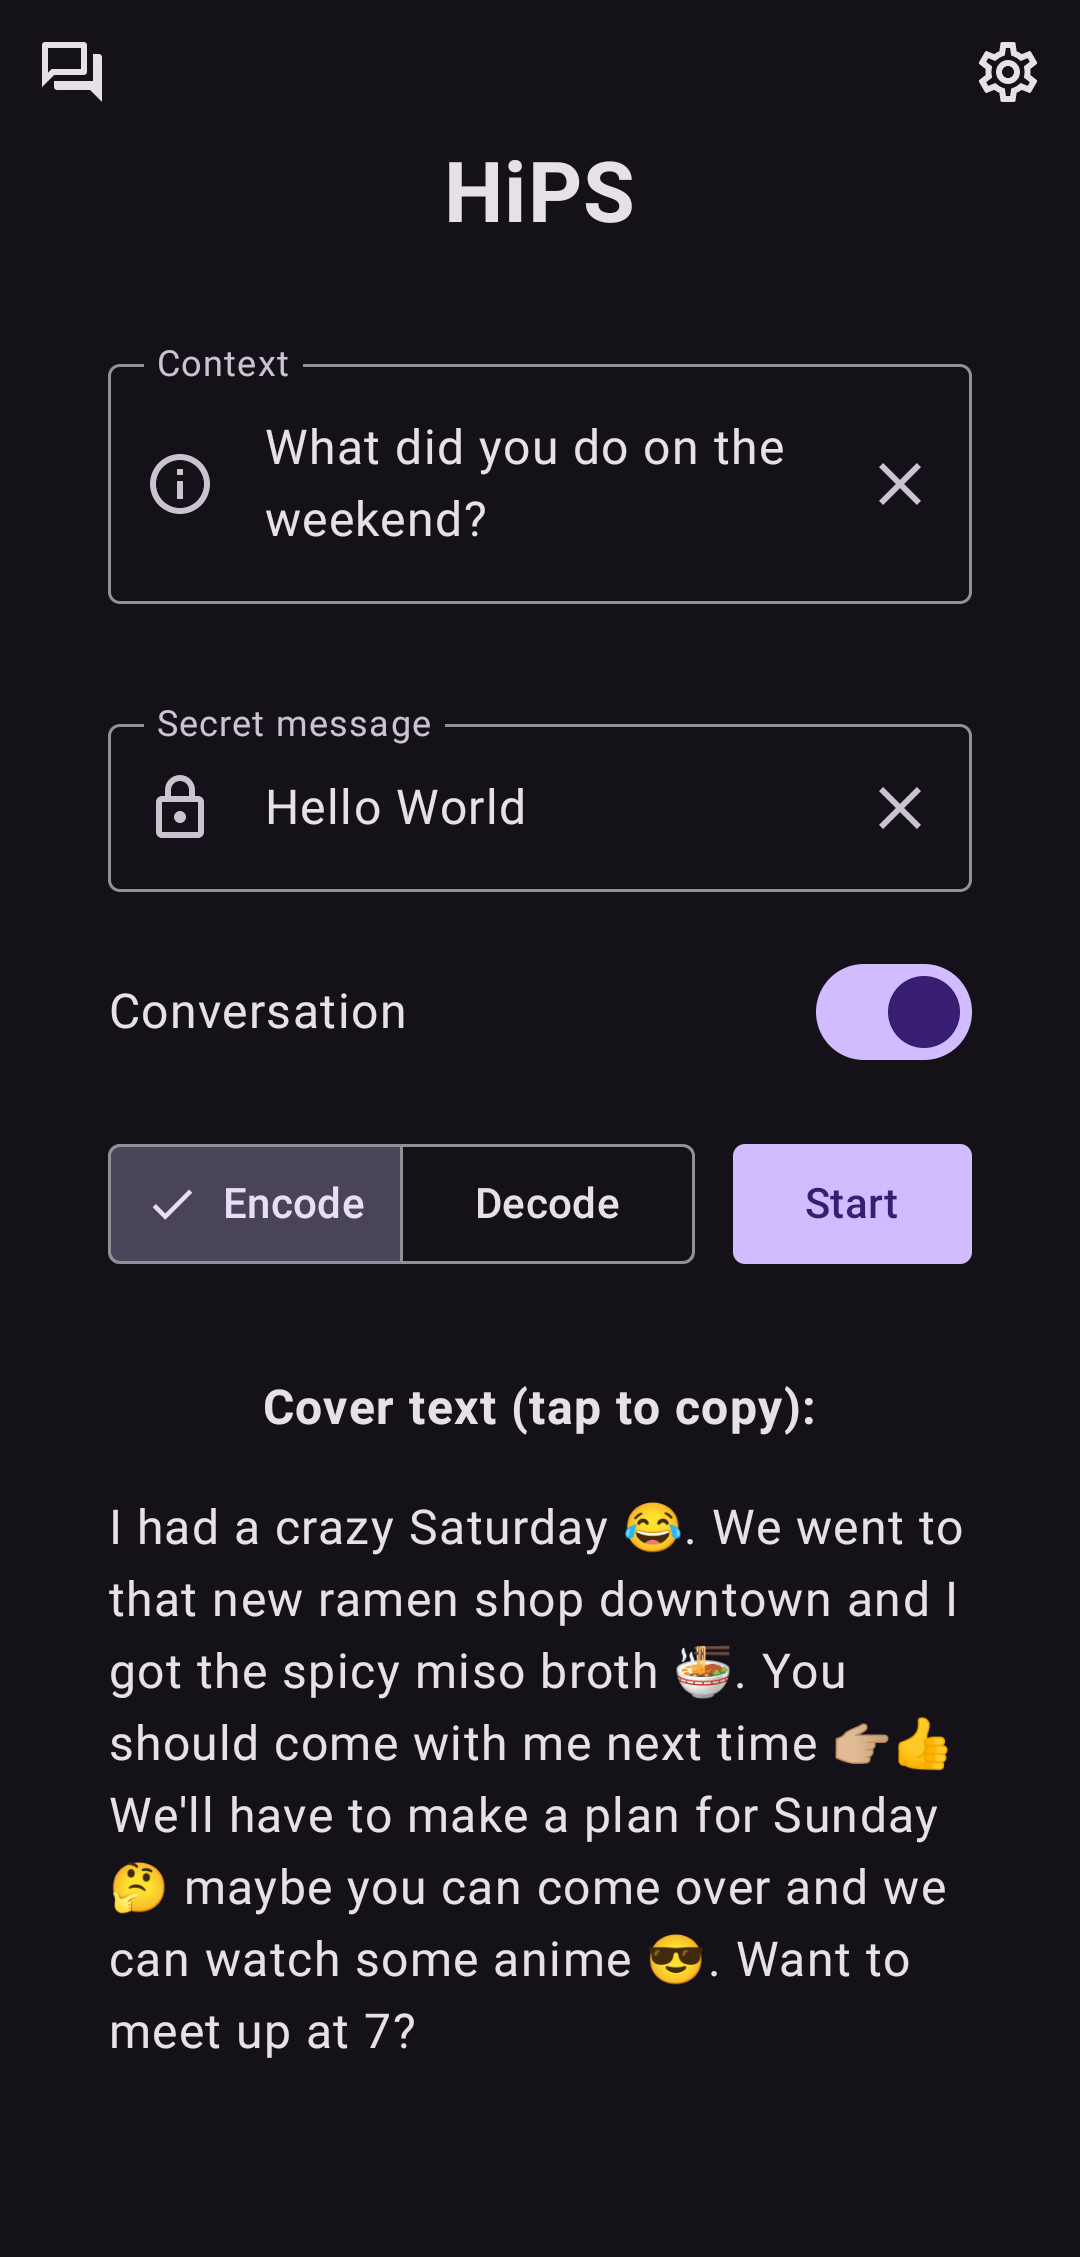
\includegraphics[width=\linewidth]{hips_home_screen_a.png}
			\caption{Encoding of a secret message.}
			\label{fig:homeScreenA}
		\end{subfigure}
        \hfill
		\begin{subfigure}{0.45\linewidth}
			\centering
			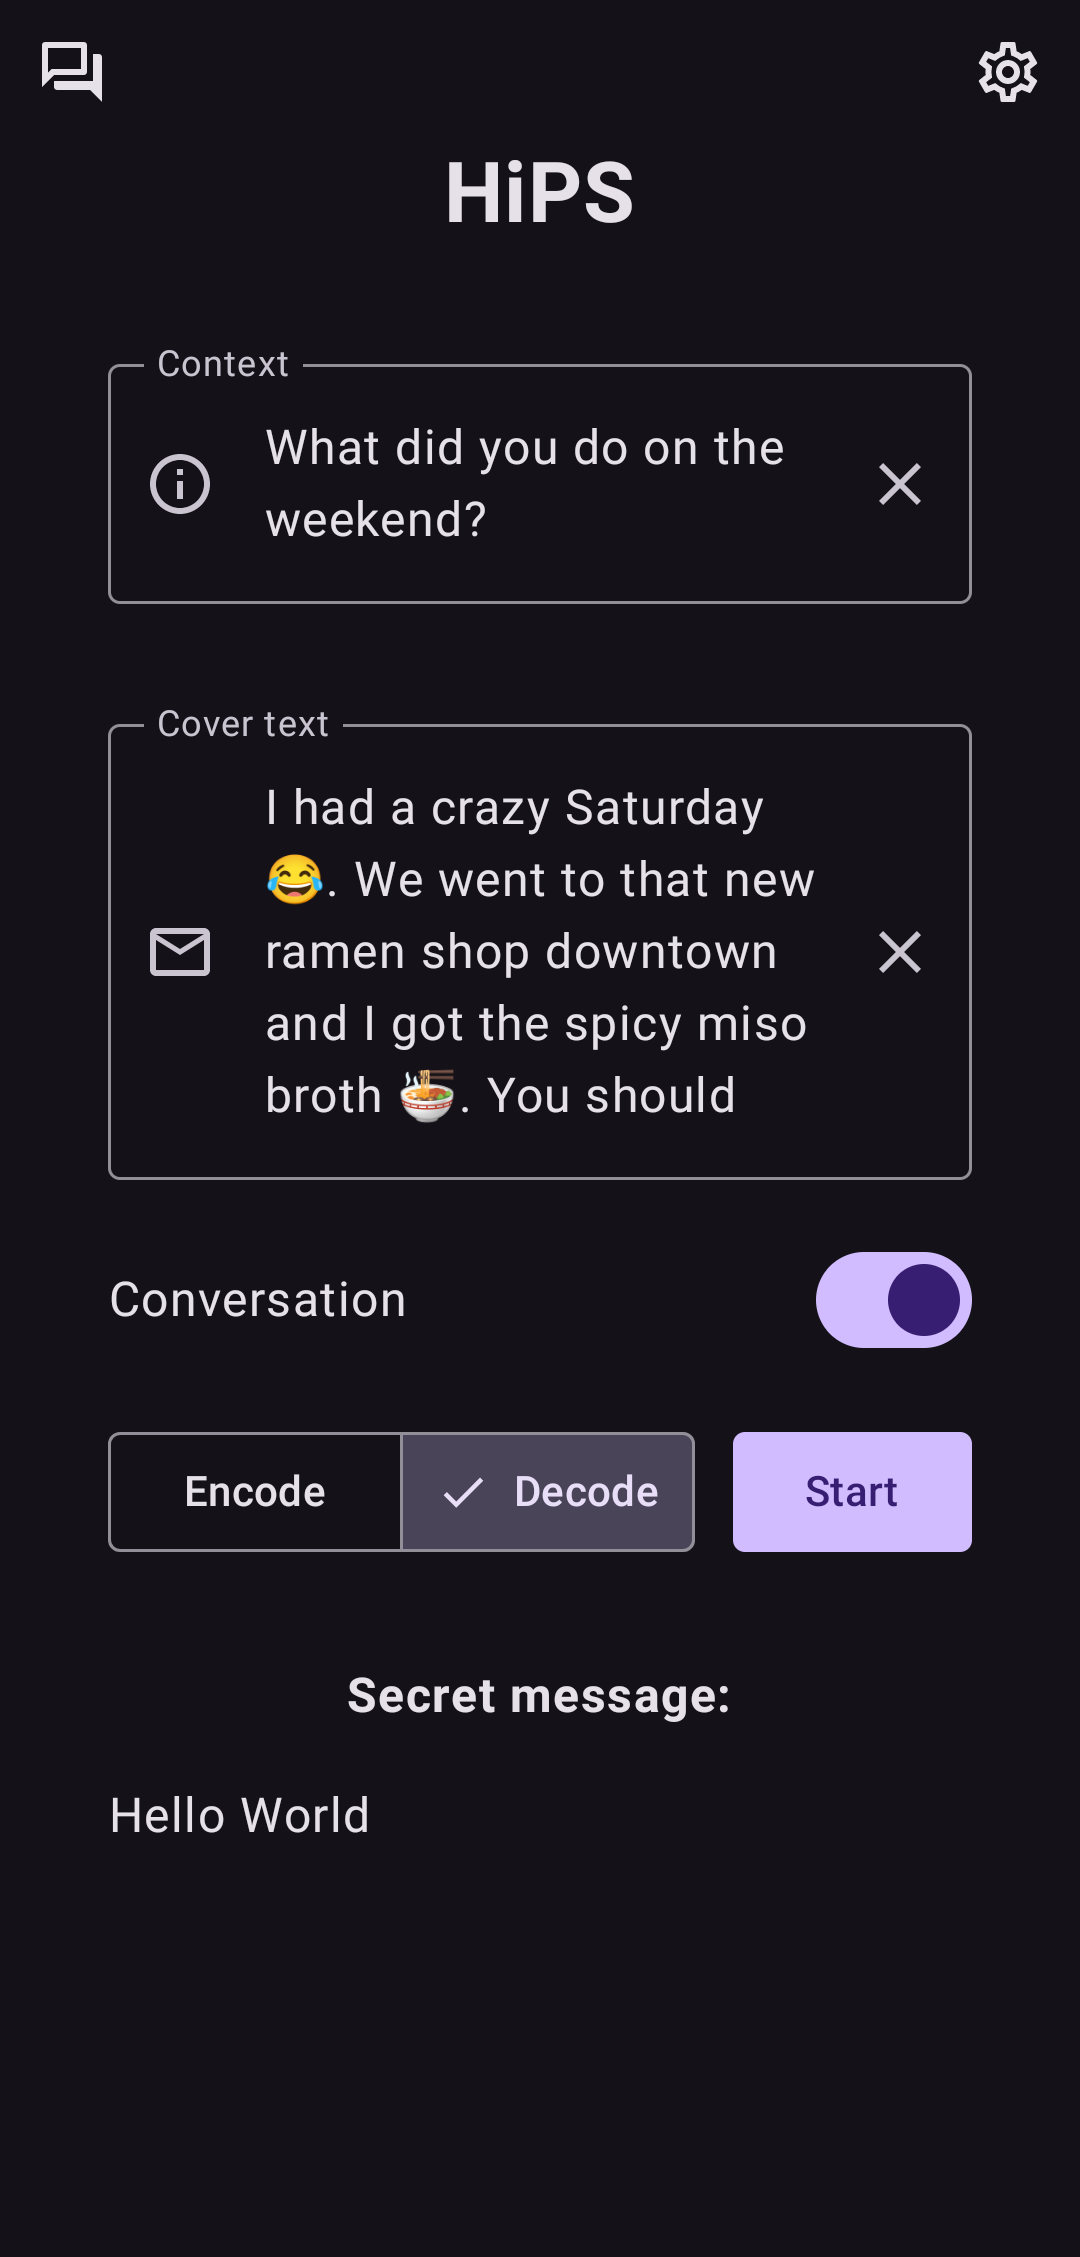
\includegraphics[width=\linewidth]{hips_home_screen_b.png}
			\caption{Decoding of a cover text.}
			\label{fig:homeScreenB}
		\end{subfigure}
		\caption[HiPS: Home screen]{Standalone functionality of HiPS on the home screen.}
		\label{fig:homeScreen}
	\end{wide}
\end{figure}

In encode mode, the input fields are for the context to generate a cover text from, and for the secret message to encode in the cover text. After pressing the start button, the cover text will be generated and displayed at the bottom. Tapping it copies it to the clipboard. In decode mode, the input fields are for the context and the cover text. After pressing the start button, the secret message will be displayed at the bottom.

The functionality of Stegasuras is replicated by toggling the conversation switch off. The cover text is then generated by \textit{completing} the context. This opens up adjacent use cases, e.g. generating a social media post to encode a secret message. When the conversation switch is toggled on, the functionality of Stegasuras is extended. The cover text is then generated by \textit{replying to} the context, i.e. the context is assumed to be a chat message. By offering this standalone functionality, we help users protect their privacy with existing instant messengers by simply copy-pasting their messages.

\subsection{Conversation screen}
\label{sec:conversationScreen}
\cref{fig:conversationScreen} shows the conversation screen. This is a demonstration of how steganography could be integrated into an instant messenger. This screen displays a list of messages, an input field and a send button. The messages are arranged as a chat conversation between two people and coloured accordingly. The input field allows the user to type in a new message, which can then be sent into the chat by pressing the send button. As this is a demo, messages are not being sent over the internet, but only stored locally. Effectively, users chat with themselves by constantly switching roles.

\begin{figure}
	\begin{wide}
		\captionsetup{width=\linewidth}
		\begin{subfigure}{0.45\linewidth}
			\centering
			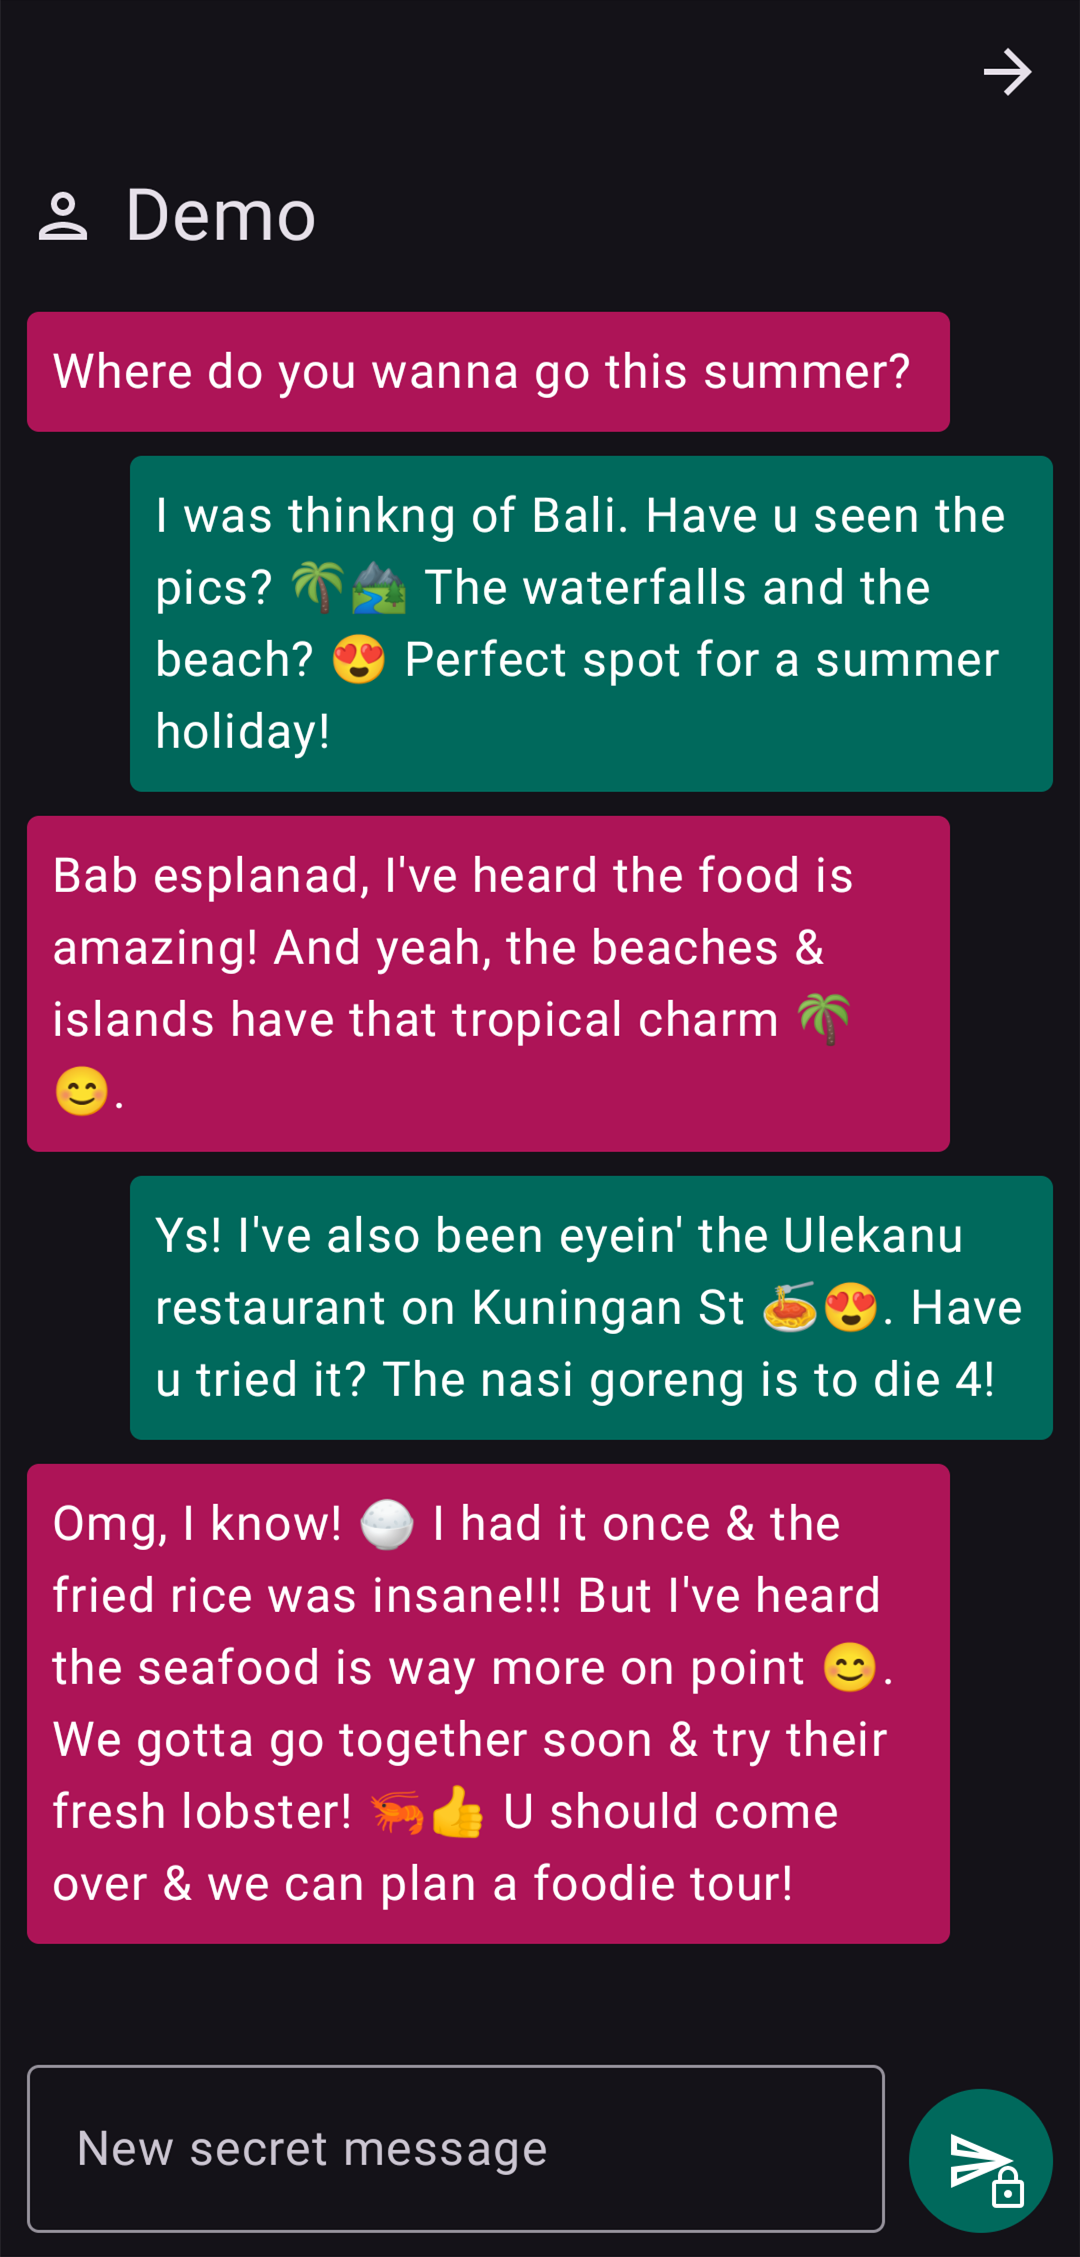
\includegraphics[width=\linewidth]{hips_conversation_screen_a.png}
			\caption{A conversation of cover texts.}
			\label{fig:conversationScreenA}
		\end{subfigure}
        \hfill
		\begin{subfigure}{0.45\linewidth}
			\centering
			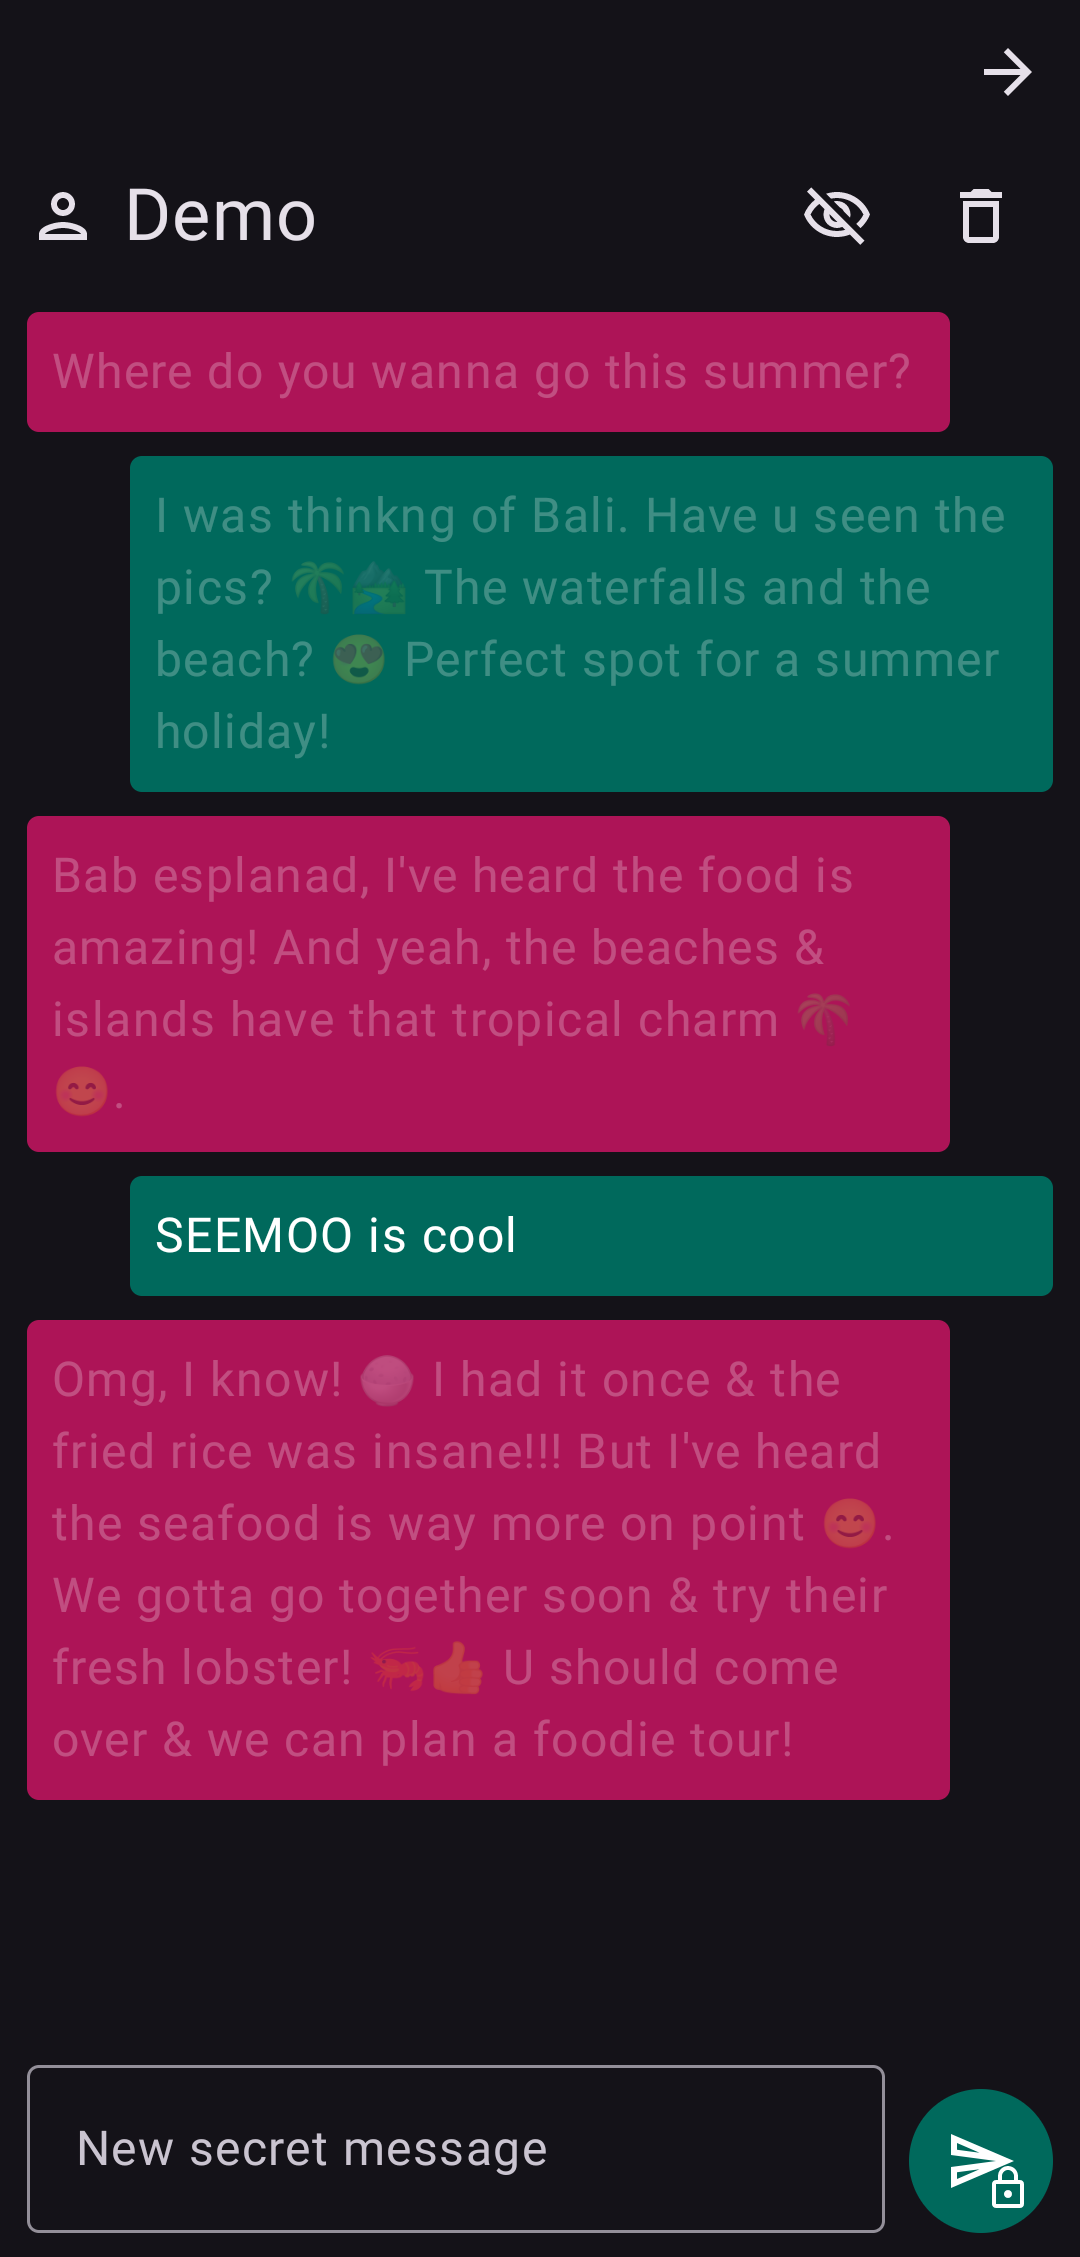
\includegraphics[width=\linewidth]{hips_conversation_screen_b.png}
			\caption{Showing a secret message.}
			\label{fig:conversationScreenB}
		\end{subfigure}
		\caption[HiPS: Conversation screen]{Steganography on the conversation screen.}
		\label{fig:conversationScreen}
	\end{wide}
\end{figure}

When the input field is blank, the send button can be short-pressed to switch roles. The current role is indicated by the send button being the same colour as the corresponding messages. This allows for sending multiple consecutive messages from the same role, i.e. for roles to not be strictly alternating. The role also switches automatically after sending a message.

The send button can be long-pressed to toggle steganography on/off. The current mode is indicated by a lock being shown or hidden inside it. If steganography is toggled on, the message in the input field is assumed to be a secret message and will be encoded into a cover text that replies to the conversation. This uses the prior messages as context. If steganography is toggled off, the message in the input field is assumed to be a plain text message and will be sent as is. This allows for arbitrary plain text messages in-between cover texts.

Messages in the chat can also be long-pressed, which highlights them as being selected. Short-pressing unselects them again. If at least one message is selected, two new buttons will be displayed at the top: Decode and delete.

The decode button can only be pressed if exactly one message is selected. This is to avoid running multiple instances of the \gls{LLM} simultaneously. Otherwise, the app process could be terminated by the Android operating system for excessive resource usage. When the decode button is pressed, it tries to decode the selected message. If decoding was successful (i.e. if the selected message was a cover text and not a plain text), the secret message will be displayed in place of the cover text. The symbol of the decode button changes to indicate that a secret message is visible. By pressing it again, the secret message and the two buttons are hidden again.

The delete button can only be pressed if the selected messages are at the end of the conversation. This is to avoid corrupting the context for decoding a message by deleting messages prior to it. When the delete button is pressed, the selected messages will be deleted and the two buttons will be hidden again.

\subsection{Settings screen}
\label{sec:settingsScreen}
\cref{fig:settingsScreen} shows the settings screen. This is where the \gls{LLM} is managed and where all parameters of our algorithms can be modified. Upon installation of our app, the user needs to download the \gls{LLM} by pressing the download button at the top of this screen. Then the \gls{LLM} can be loaded into or unloaded from memory by pressing the start/stop button below the download button. Pressing this button is only necessary after downloading the \gls{LLM} when using our app for the first time. Afterwards, the \gls{LLM} is automatically loaded on startup.

\begin{figure}
	\begin{wide}
		\captionsetup{width=\linewidth}
		\begin{subfigure}{0.3\linewidth}
			\centering
			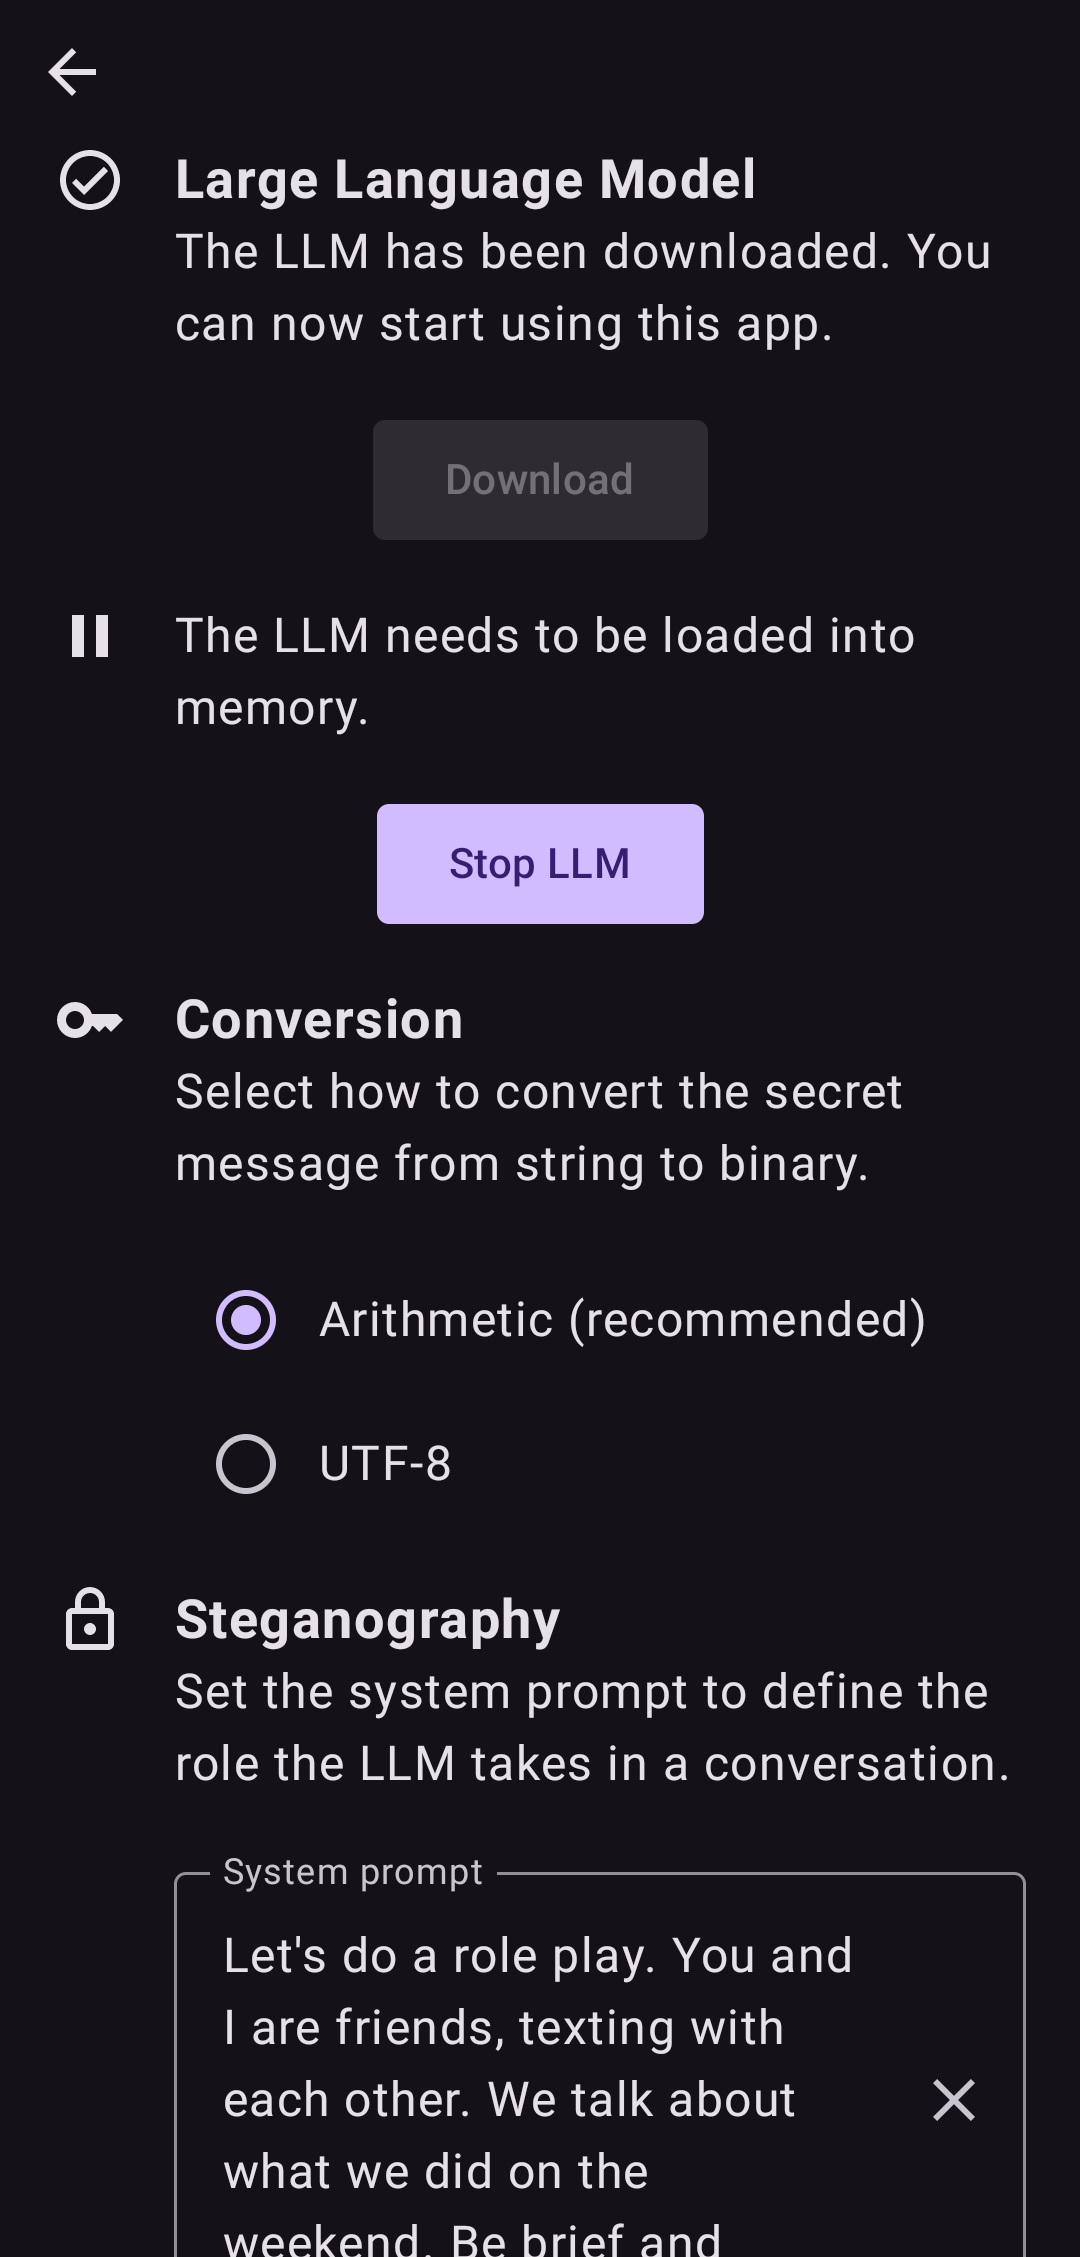
\includegraphics[width=\linewidth]{hips_settings_screen_a.png}
			\caption{Download button, start button and binary conversion mode.}
			\label{fig:settingsScreenA}
		\end{subfigure}
        \hfill
        \begin{subfigure}{0.3\linewidth}
			\centering
			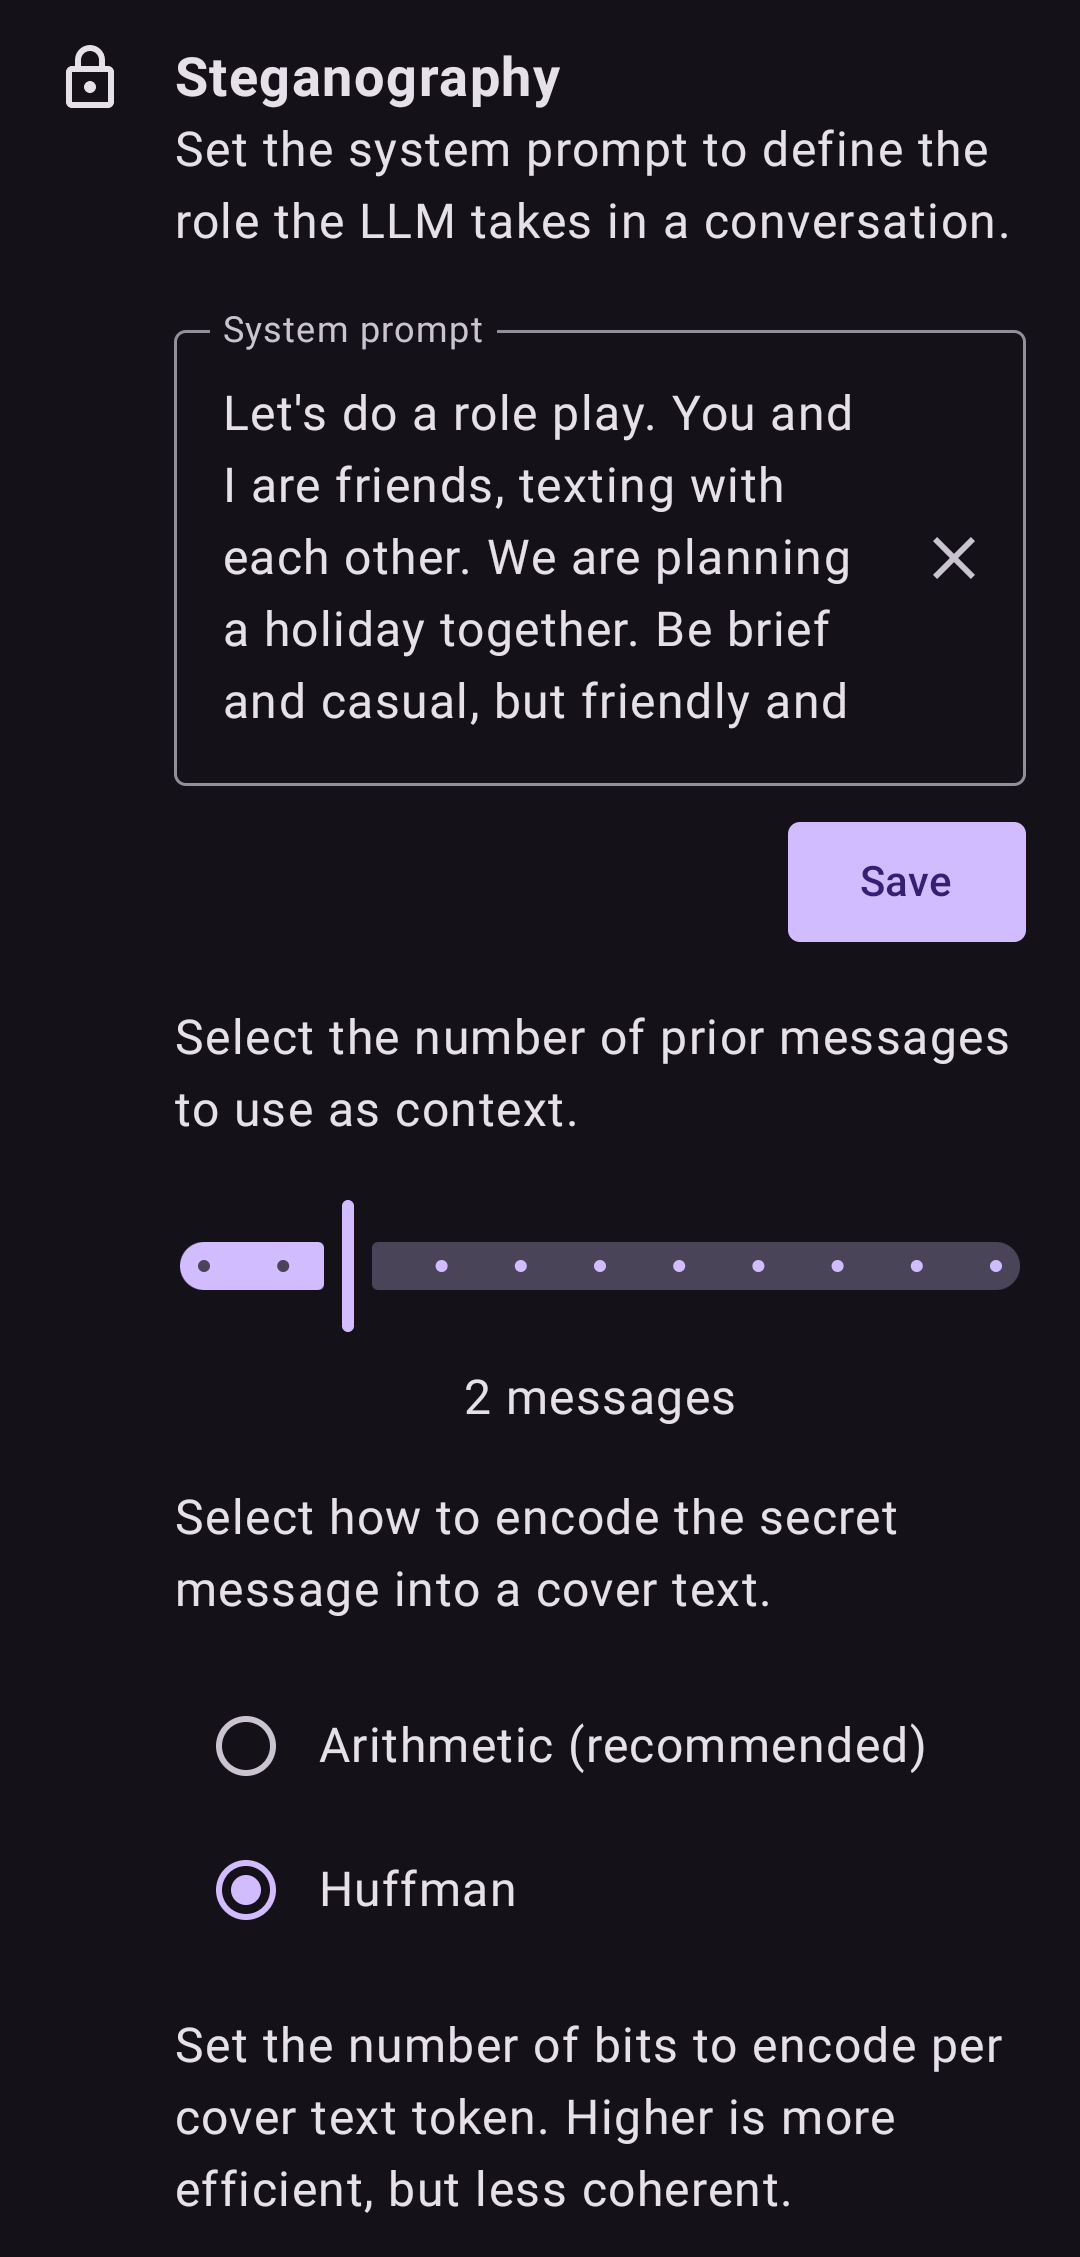
\includegraphics[width=\linewidth]{hips_settings_screen_b.png}
			\caption{System prompt, context length and steganography mode.}
			\label{fig:settingsScreenB}
		\end{subfigure}
        \hfill
        \begin{subfigure}{0.3\linewidth}
			\centering
			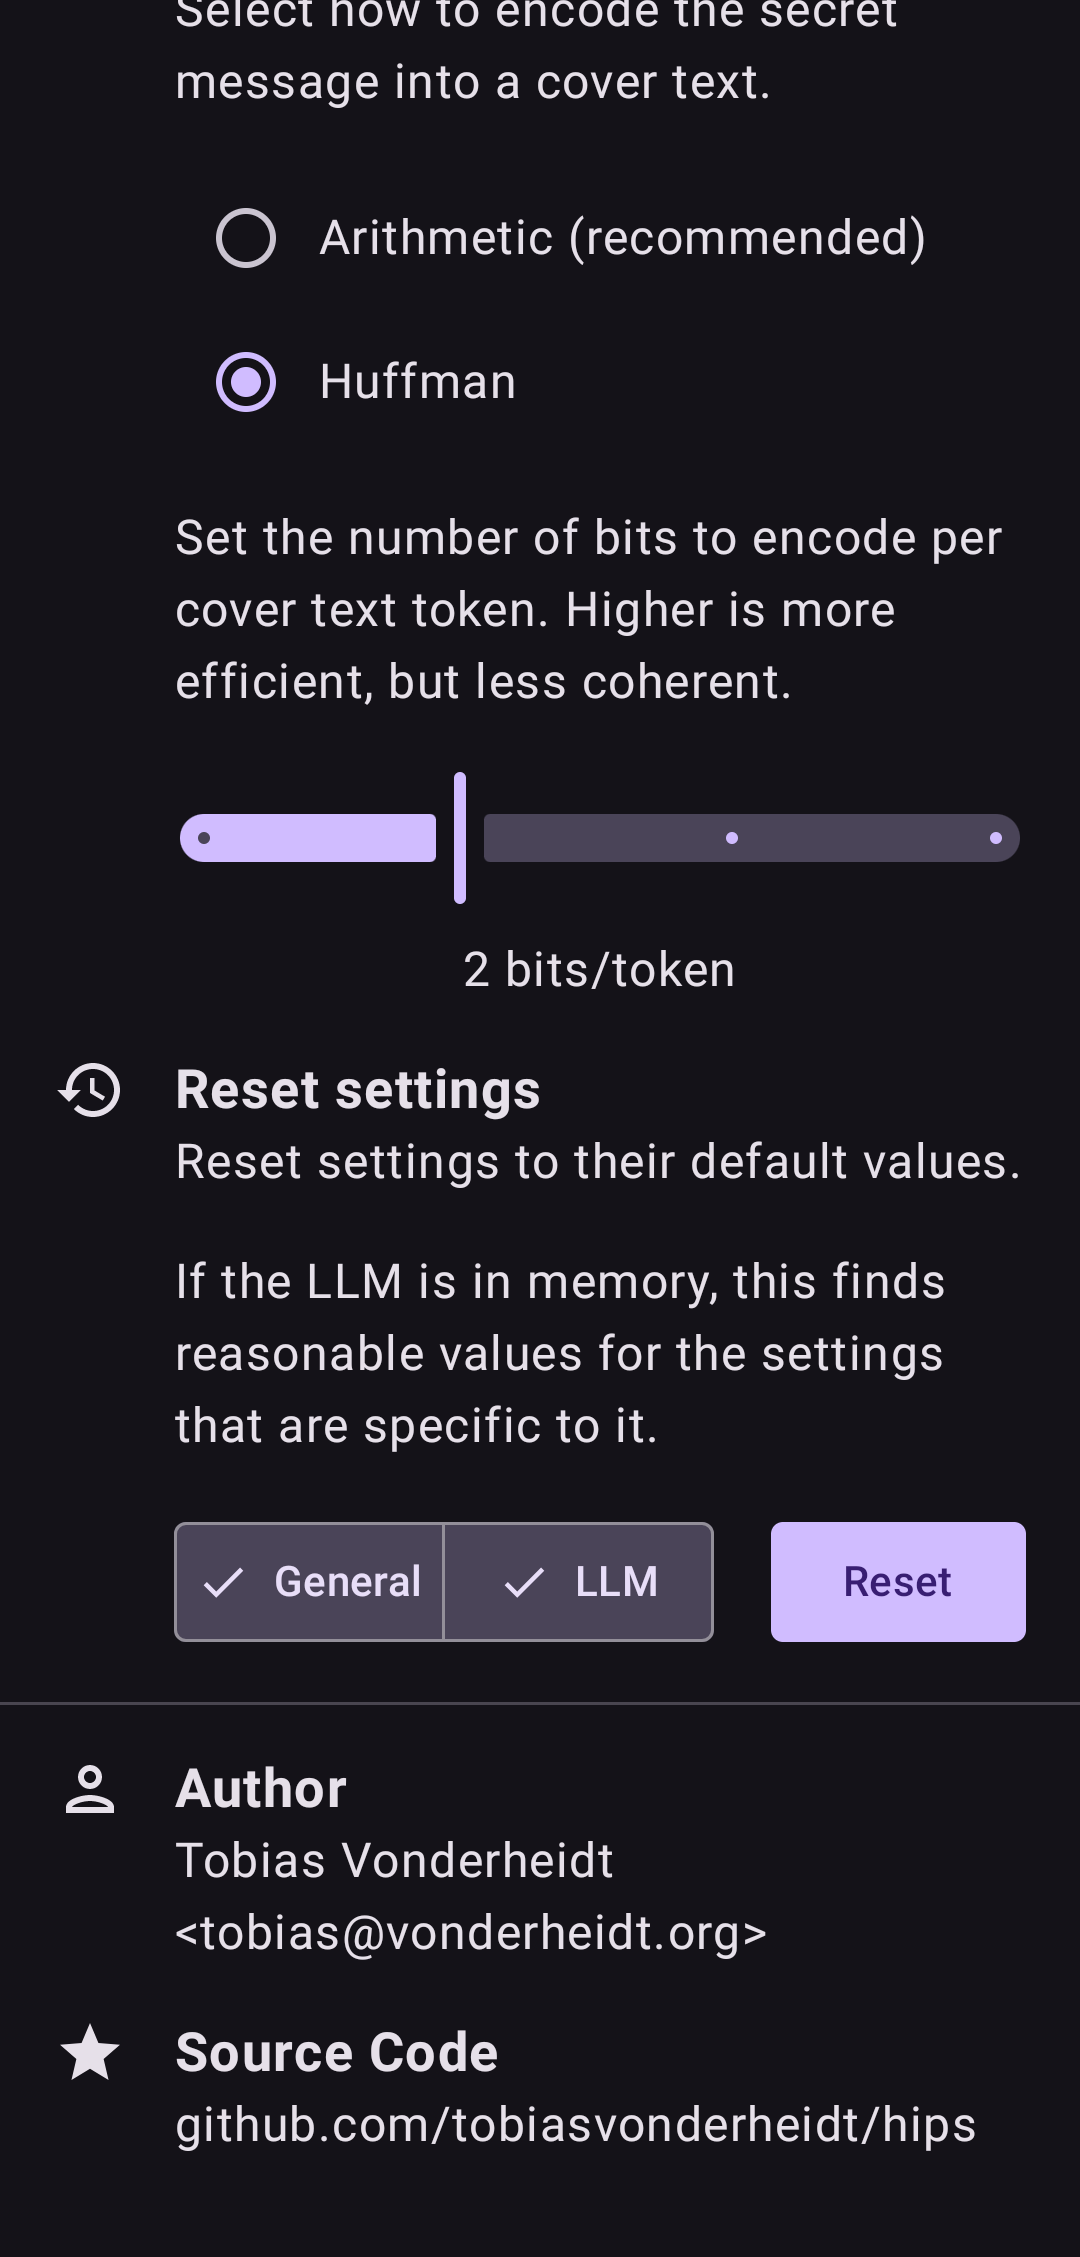
\includegraphics[width=\linewidth]{hips_settings_screen_c.png}
			\caption{Algorithm-specific settings for Huffman coding and reset options.}
			\label{fig:settingsScreenC}
		\end{subfigure}
		\caption[HiPS: Settings screen]{The settings screen.}
		\label{fig:settingsScreen}
	\end{wide}
\end{figure}

Below these buttons, there are various selectors, sliders and input fields for the parameters of our algorithms. They are arranged in the order of corresponding steps during the encoding of a secret message. First there is a selector for the conversion mode, i.e. for how to convert the secret message from string to binary. It offers \lstinline|Arithmetic (recommended)|, \lstinline|Huffman| and \lstinline|UTF-8| as options. \lstinline|UTF-8| serves as a baseline as it doesn't compress the secret message, while \lstinline|Arithmetic| compresses it using the \gls{LLM} and \lstinline|Huffman| compresses it without using the \gls{LLM} (see \cref{sec:binaryConversionAndCompression} for details).

This is followed by an input field for a system prompt. This is a natural language command that can be passed to the \gls{LLM} to influence its behaviour (see \cref{sec:creatingAConversationBetweenCoverTexts} for details). This is relevant for the conversation screen, and for the home screen if the conversation switch there is toggled on.

Afterwards, there is a slider to select a number of messages between 0 and 10. This is the number of prior messages to use as context on the conversation screen. While values 1 to 10 are used as is, 0 is interpreted as \lstinline|All messages|. This means all prior messages will be used as context to generate the next cover text from. We recommend setting this slider to a low value in the 1-10 range to limit resource usage.

Furthermore, we have a selector for the steganography algorithm. It offers \lstinline|Arithmetic (recommended)| and \lstinline|Huffman| as options. Parameters specific to the selected algorithm can be set using sliders below this selector (see \cref{sec:steganographyEncodingDecoding} for details): For \lstinline|Arithmetic|, there are three parameters called \lstinline|temperature|, \lstinline|topK| and \lstinline|precision|. Both \lstinline|topK| and \lstinline|precision| are only visible when the \gls{LLM} is in memory, as they are specific to the \gls{LLM}. For \lstinline|Huffman|, there is one parameter called \lstinline|bitsPerToken|.

Lastly, there is a button to reset all settings to their default values. It comes with a selector for whether to reset either only general settings, only settings that are specific to the \gls{LLM}, or both. When the \gls{LLM} is in memory, settings specific to it will be reset to sensible defaults. Otherwise, they are reset to 0.

\section{Java Native Interface}
\label{sec:javaNativeInterface}
We chose llama.cpp as the framework to run our \gls{LLM} with. Since this is a C++ library, we need a way to integrate C++ code into our Kotlin-based Android app. This is facilitated by the \gls{JNI}. It allows us to declare Kotlin functions as \lstinline|external|, signalling that their implementation is done in C++ rather than Kotlin. Arguments and return values can then be passed back and forth between Kotlin and C++.

Listings~\ref{lst:jniKotlin} and~\ref{lst:jniCpp} show examples for the Kotlin and C++ sides of the \gls{JNI}. On the Kotlin side, we implement the \lstinline|LlamaCpp| class to represent the \gls{LLM} instance. More specifically, \lstinline|LlamaCpp| is an \lstinline|object|. This is the Kotlin syntax for a singleton class. Multiple instances of the \gls{LLM} are avoided this way. On the C++ side, we only have implementations of functions declared \lstinline|external| in Kotlin, which generally are wrappers for llama.cpp function calls. Inputs and outputs need to be converted between Kotlin and C++ data types, but most logic is implemented in Kotlin. While this design decision may introduce performance drawbacks (see \cref{sec:performance}), it makes maintenance significantly easier.

% Add some space on top of listing to match bottom
\vspace{0.25cm}

\begin{lstlisting}[caption={[JNI: Kotlin side]{Example for the Kotlin side of the \gls{JNI}: State management for the \gls{LLM} using a function declared \lstinline|external| at the end.}}, label={lst:jniKotlin}]
object LlamaCpp {
    @Volatile
    private var model = 0L

    fun isInMemory(): Boolean {
        return model != 0L
    }

    fun startInstance() {
        if (isInMemory()) {
            return
        }

        synchronized(lock = this) {
            if (!isInMemory()) {
                model = loadModel()
            }
        }
    }

    private external fun loadModel(path: String): Long
}
\end{lstlisting}

% Move following paragraphs here to avoid page break in next listing
On the Kotlin side, the \gls{LLM} is loaded into memory by calling the \lstinline|loadModel| function with the path to a \lstinline|.gguf| file as a string argument. This function is declared \lstinline|external|, so its implementation is in C++. On the C++ side, the Kotlin string is converted to a C++ string via the \gls{JNI}. In turn, the \lstinline|llama_model_load_from_file| function of llama.cpp is called, which takes the file path as C++ string and some default parameters as arguments. This returns the memory address of the \gls{LLM} as a pointer. Pointers only exist in C++, but can be cast to Kotlin long numbers as both are 64 bits in size. Therefore, \lstinline|loadModel| returns a Kotlin long number. This is stored in the attribute \lstinline|model| of the \lstinline|LlamaCpp| object, so the state of the \gls{LLM} can be managed: If \lstinline|model| is \lstinline|0L|, the \gls{LLM} is not in memory. Otherwise it is and can be referenced via this attribute.

This enables us to implement any further logic in Kotlin. For example, the \lstinline|startInstance| function shown in Listing~\ref{lst:jniKotlin} loads of the \gls{LLM} in a thread-safe manner by implementing a double-checked locking mechanism~\cite{ishizakiTransformingJavaPrograms2014}. This is commonly used with singleton classes in Java, and by extension, Kotlin. Unloading the \gls{LLM} mirrors this. Other interactions with the \gls{LLM} are implemented similarly.

% Add some space on top of listing to match bottom
\vspace{0.25cm}

\begin{lstlisting}[caption={[JNI: C++ side]{Example for the C++ side of the \gls{JNI}: Implementation of the function declared \lstinline|external| in Listing~\ref{lst:jniKotlin}.}}, label={lst:jniCpp}]
extern "C" JNIEXPORT jlong JNICALL Java_org_vonderheidt_hips_utils_LlamaCpp_loadModel(JNIEnv* env, jobject /* thiz */, jstring jPath) {
    jboolean isCopy = true;

    const char* cppPath = env -> GetStringUTFChars(jPath, &isCopy);

    llama_model_params params = llama_model_default_params();

    llama_model* cppModel = llama_model_load_from_file(cppPath, params);

    env -> ReleaseStringUTFChars(jPath, cppPath);

    auto jModel = reinterpret_cast<jlong>(cppModel);

    return jModel;
}
\end{lstlisting}

\section{Token generation with llama.cpp}
\label{sec:tokenGenerationWithLlamaCpp}
\gls{HiPS} uses the popular llama.cpp framework to run \glspl{LLM} locally. We explain how token generation works with llama.cpp, i.e. how the \gls{LLM} generates text. We focus on the abstractions needed to work with llama.cpp, omitting any more general concepts. Most of this explanation is based on a great blog post by Omri Mallis~\cite{mallisUnderstandingHowLLM2023} and the examples given in the llama.cpp GitHub repository~\cite{gerganovGgerganovLlamacpp2024}. \cref{fig:llamaCppHighLevelFlow} shows the high-level flow we need to understand.

\begin{figure}
    \begin{wide}
        \captionsetup{width=\linewidth}
        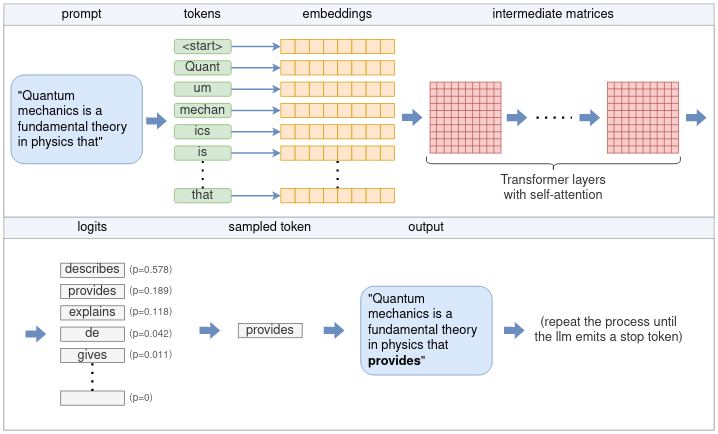
\includegraphics[width=\linewidth]{llama_cpp_high_level_flow.png}
        \caption[llama.cpp: Token generation]{High-level flow of token generation in llama.cpp. Taken from~\cite{mallisUnderstandingHowLLM2023}.}
        \label{fig:llamaCppHighLevelFlow}
    \end{wide}
\end{figure}

Fundamentally, \glspl{LLM} iteratively complete any text they are given as input~\cite{mallisUnderstandingHowLLM2023}. We call this input a prompt. The generated completion is returned as output. We call this output the response. In \cref{fig:llamaCppHighLevelFlow}, the prompt is "Quantum mechanics is a fundamental theory of physics that" and the response after one iteration is "provides"~\cite{mallisUnderstandingHowLLM2023}. The following paragraphs will explain what happens that iteration.

First, we need to understand an important distinction: The \gls{LLM} and its state. In the llama.cpp source code, the \gls{LLM} is called \lstinline|model|. Its state is called \lstinline|ctx| (short for context)~\cite{gerganovGgerganovLlamacpp2024}. The \lstinline|model| itself is stateless. This can be demonstrated by its idempotence: Consider one instance of a \lstinline|model| with an empty \lstinline|ctx|. When it is given a prompt, it will return a response. Reset the \lstinline|ctx| so it is empty again. If you give it the same prompt now, you will receive the same response again. Resetting the \lstinline|ctx| is important in our implementation to ensure reproducible results.

A \lstinline|ctx| takes the memory address of a \lstinline|model| as argument when being created~\cite{gerganovGgerganovLlamacpp2024}. Thereby, it is attached to the \lstinline|model| instance. Token generation only needs to access the \lstinline|ctx|. Resetting the \lstinline|ctx| works by unloading it from memory and loading a new \lstinline|ctx| attached to the same \lstinline|model| instance into memory. The implementation is analogous to loading and unloading the \gls{LLM} as shown in \cref{sec:javaNativeInterface}. However, the following paragraphs will only refer to the \gls{LLM} for readability, abstracting the \lstinline|ctx| away.

The \gls{LLM} starts processing the prompt by tokenizing it. This means that the prompt is not just split into words, but dismantled further into sub-word units called tokens~\cite{mallisUnderstandingHowLLM2023}. In \cref{fig:llamaCppHighLevelFlow}, for example the word "Quantum" is composed of the tokens "Quant" and "um". A token can be represented as a string, which is depicted in~\cref{fig:llamaCppHighLevelFlow}, or as an integer, which is then called the token ID~\cite{mallisUnderstandingHowLLM2023}. After tokenization, the \gls{LLM} works with token IDs. But for readability, we will mostly refer to them as tokens.

A common tokenization algorithm is \gls{BPE}~\cite{sennrichNeuralMachineTranslation2016}. Popular tokenizers using \gls{BPE} include Google's SentencePiece~\cite{googleGoogleSentencepiece2024}, which is used in Stegasuras~\cite{zieglerHarvardnlpNeuralSteganography2025,zieglerStegasuras2025}, and OpenAI's TikToken~\cite{openaiOpenaiTiktoken2025}, which is used in our \gls{LLM} of choice, Llama 3.2 1B~\cite{metaMetallamaLlamamodels2025}.

In llama.cpp, the tokens to be processed are stored in a separate data structure called a \lstinline|batch|. During the first iteration, the batch contains all tokens of the prompt. During subsequent iterations, the batch only contains the last sampled token~\cite{gerganovGgerganovLlamacpp2024}.

To complete the prompt, the \gls{LLM} needs to predict which tokens are likely to come next. To be comparable, the tokens need to be converted into a more structured representation. Each token in the prompt is converted into a vector, called an embedding~\cite{mallisUnderstandingHowLLM2023}. These vectors are then stacked to form the embedding matrix~\cite{mallisUnderstandingHowLLM2023}. \cref{fig:llamaCppEmbedding} shows the embedding matrix in detail. Its dimensions are \lstinline|n_tokens| $\times$ \lstinline|n_embd|. \lstinline|n_tokens| is the number of tokens in the prompt. \lstinline|n_embd| is the dimension of the vectors representing the tokens, which is specific to the \gls{LLM}~\cite{mallisUnderstandingHowLLM2023}.

\begin{figure}
    \begin{wide}
        \centering
        \captionsetup{width=\linewidth}
        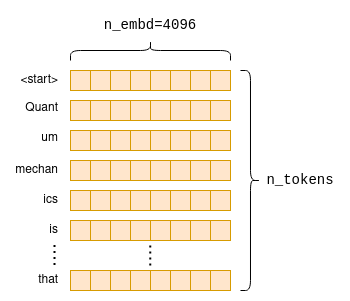
\includegraphics[width=0.5\linewidth]{llama_cpp_embedding.png}
        \caption[llama.cpp: Embedding matrix]{Details of the embedding matrix in llama.cpp. \lstinline|n_embd| is specific to the \gls{LLM} (the value depicted here is for Llama 2). Taken from~\cite{mallisUnderstandingHowLLM2023}.}
        \label{fig:llamaCppEmbedding}
    \end{wide}
\end{figure}

With the prompt effectively converted into a matrix representation, the \gls{LLM} can now apply \textit{transformations} to it, i.e. multiply it with a series of matrices. \cref{fig:llamaCppHighLevelFlow} depicts this as "Transformer layers with self-attention". This is the core of the \textit{Transformer} architecture, which is the basis for most \glspl{LLM} today~\cite{vaswaniAttentionAllYou2023}. Different variants of the Transformer architecture exist, namely encoder-decoder or decoder-only~\cite{mallisUnderstandingHowLLM2023}. They each come with their own strengths and weaknesses, the discussion of which is out of scope for this thesis. For us, it is only relevant that we want to support as many \glspl{LLM} as possible. This means we have to check if an encoding step is required before performing the decoding step. Fortunately, llama.cpp abstracts this away behind a simple function call each~\cite{gerganovGgerganovLlamacpp2024}. This was shown earlier in Listing~\ref{lst:llamaCpp}. The result of these transformations is a matrix of logits, i.e. of unnormalized probabilities for the prediction of the next token~\cite{mallisUnderstandingHowLLM2023}. \cref{fig:llamaCppLogits} shows the logits matrix in detail. Its dimensions are \lstinline|n_tokens| $\times$ \lstinline|n_vocab|. \lstinline|n_vocab| is the vocabulary size specific to the \gls{LLM}, i.e. the number of tokens it knows~\cite{mallisUnderstandingHowLLM2023}.

\begin{figure}
    \begin{wide}
        \captionsetup{width=\linewidth}
        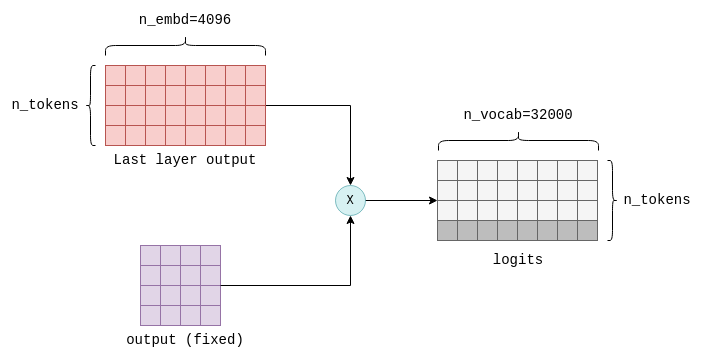
\includegraphics[width=\linewidth]{llama_cpp_logits.png}
        \caption[llama.cpp: Logit matrix]{Details of the logit matrix in llama.cpp. Also shown is the last transformation layer, i.e. the last intermediate matrix being multiplied with a fixed "output" matrix. This is not to be confused with the output of the \gls{LLM} as defined earlier. Taken from~\cite{mallisUnderstandingHowLLM2023}.}
        \label{fig:llamaCppLogits}
    \end{wide}
\end{figure}

Each row of the logit matrix corresponds to a token in the prompt. It contains the logits for every token in the vocabulary to follow this token of the prompt. In other words, only the last row of the logit matrix is relevant for us, as it contains the logits for the last token of the prompt~\cite{mallisUnderstandingHowLLM2023}. This is highlighted in \cref{fig:llamaCppLogits}. Generally, these logits will be normalized using a softmax function (see \cref{sec:theGenericAlgorithm} for details). Only then they are interpretable as probabilities~\cite{mallisUnderstandingHowLLM2023,turnerIntroductionTransformers2024}.

Now we need to sample a token to complete the prompt with, based on the probabilities we just calculated~\cite{mallisUnderstandingHowLLM2023}. We will implement our own sampling logic to perform steganography, i.e. to encode a secret message into a cover text by sampling certain tokens (see \cref{sec:arithmeticCoding,sec:huffmanCoding} for details). To do this, we need to understand several general-purpose sampling methods. The simplest is called greedy sampling. Greedy sampling always selects the token with the highest probability~\cite{mallisUnderstandingHowLLM2023}. Other common approaches are temperature sampling and top-k sampling~\cite{mallisUnderstandingHowLLM2023}. In temperature sampling, the probabilities are scaled with $1/temperature$ to modify their distribution. For $temperature < 1$, the distribution gets steeper around the most likely token. This makes the \gls{LLM} responses more coherent. For $temperature > 1$, the distribution gets flatter. This makes the \gls{LLM} responses less coherent ("more creative")~\cite{mallisUnderstandingHowLLM2023}. Top-k sampling only considers the tokens with the k highest probabilities~\cite{mallisUnderstandingHowLLM2023}.

When a token is sampled, it is appended to the prompt to construct the response~\cite{mallisUnderstandingHowLLM2023}. The full response is built iteratively, so this output is used as input for the next iteration. This is also called autoregressive~\cite{mallisUnderstandingHowLLM2023}. Iteration stops when the \gls{LLM} samples a special end-of-generation token~\cite{gerganovGgerganovLlamacpp2024}. While the response in principle is ready now, it is still represented as token IDs. Before being displayed to the user as a string, it needs to be detokenized~\cite{mallisUnderstandingHowLLM2023}. The response after one iteration is shown in \cref{fig:llamaCppHighLevelFlow}, after sampling the token "provides".

\section{Algorithms}
\label{sec:algorithms}
Our app implements algorithms to perform steganography in two steps:
\begin{itemize}
    \item Convert the secret message from string to binary, compressing it in the process.
    \item Generate a cover text by completing a given context with the \gls{LLM}, thereby encoding the secret message bits.
\end{itemize}

This can be viewed as a generic algorithm with exchangeable implementations for each of the two steps. For the first step, we implement UTF-8 conversion, Huffman compression and Arithmetic compression. For the second step, we implement Huffman coding and Arithmetic coding. We first discuss the generic algorithm, then the different implementations for each step. This is intended as a high-level overview to support documentation of our code.

\subsection{The generic algorithm}
\label{sec:theGenericAlgorithm}
The algorithms demonstrated by Stegasuras~\cite{zieglerNeuralLinguisticSteganography2019} can be viewed as different implementations of a single generic algorithm, differing only in the logic used to encode information during token sampling. We explain the generic algorithm here.

To \textbf{encode} the bits of a secret message into a cover text using a context, we tokenize the context first. We let the \gls{LLM} generate cover text tokens in a loop. This loop terminates when all bits are encoded and the last sentence of the cover text is finished. In every iteration, we let the \gls{LLM} calculate logits: First using the context tokens, then using the last cover text token we sampled. As logits can generally assume negative values, they need to be normalized to the $ [0, 1] $ interval to be interpretable as probabilities. This is done using a softmax function~\cite{turnerIntroductionTransformers2024}. \cref{eqn:softmax} shows a softmax function ($p_i$ = probability of token i, $l_i$ = logit of token i, $n_{vocab}$ = vocabulary size of the \gls{LLM}). It applies the exponential function to transform the logits to non-negative values. This is suitable as the exponential function is strictly monotonous in growth, therefore maintaining the order of the associated tokens.

\begin{align}
	p_i = \frac{\exp(l_i)}{\sum_{j=1}^{n_{vocab}} \exp(l_j)}
	\label{eqn:softmax}
\end{align}

To avoid early termination, we need to manually suppress end-of-generation tokens by setting their probability to 0. Otherwise, we may render our secret message unrecoverable by not encoding all of its bits.

If there are secret message bits left to encode, the algorithm-specific sampling logic is applied (see \cref{sec:arithmeticCoding,sec:huffmanCoding}). It samples cover text tokens based on the secret message bits using these probabilities. Otherwise, greedy sampling is applied to finish the last sentence of the cover text (see \cref{sec:finishingTheLastSentence}). After the last iteration, the sampled cover text tokens are detokenized to return the cover text.

To \textbf{decode} a cover text back into a secret message bits using a context, we calculate the same probabilities as during encoding: We tokenize both context and cover text. In a loop through the cover text tokens, we let the \gls{LLM} calculate logits. Again first using the context tokens, then using the current cover text token. Now we only need to inverse the algorithm-specific sampling logic, deriving the secret message bits from the cover text tokens. After processing all cover text tokens, we return the binary secret message.

\subsection{UTF-8}
\label{sec:utf8}
To convert the secret message from string to binary, we implement UTF-8 encoding. We chose UTF-8 as it is the most popular Unicode encoding: Around 90\% of all text on the internet is encoded in UTF-8~\cite{gleaveMakingCompressionAlgorithms2017}. It doesn't compress the secret message, but represents every character with one to four bytes instead~\cite{gleaveMakingCompressionAlgorithms2017}. This makes cover texts significantly longer. Therefore, it serves as a baseline to compare Arithmetic and Huffman compression to.

\subsection{Binary conversion and compression}
\label{sec:binaryConversionAndCompression}
We implement three methods to convert the secret message back and forth between its string and binary representations: UTF-8 conversion, Huffman compression and Arithmetic compression.

\subsubsection{Huffman compression}
\label{sec:huffmanCompression}
Adding Huffman compression is our first extension of Stegasuras~\cite{zieglerNeuralLinguisticSteganography2019}. Huffman compression is popular because of its ability to compress data to near entropy~\cite{huffmanMethodConstructionMinimumRedundancy1952}. We use it to illustrate the benefits and drawbacks of Arithmetic compression (see \cref{sec:arithmeticCompression}) in comparison to many other similar algorithms.

We define some data structures as generic classes for reuse in Huffman coding (see \cref{sec:huffmanCoding}). Huffman compression constructs a binary tree, the Huffman tree, which is composed of nodes~\cite{huffmanMethodConstructionMinimumRedundancy1952}. Each node stores an \textit{element}, the element's \textit{frequency}, and its own left and right child nodes as attributes~\cite{huffmanMethodConstructionMinimumRedundancy1952}. For compression, elements and frequencies are characters and their frequencies in the secret message. For steganography, they are tokens and their probabilities. Nodes are compared by frequency~\cite{huffmanMethodConstructionMinimumRedundancy1952}.

We use a Java PriorityQueue to construct the Huffman tree iteratively. Initially, it contains all nodes representing elements. In each iteration, we remove the two nodes with the lowest frequencies. We create a new parent node for them with the sum of their frequencies, but no element. The new node gets inserted back into the priority queue. Iteration ends when there is only one node left, which becomes the root node~\cite{huffmanMethodConstructionMinimumRedundancy1952}. Only now is the Huffman tree a binary tree. Its leaf nodes represent the elements. Above them, the new nodes have been inserted. They don't represent elements, but store the cumulated frequencies of their sub-trees~\cite{huffmanMethodConstructionMinimumRedundancy1952}.

Huffman codes are generated by traversing the Huffman tree from top to bottom, interpreting a left turn as a 0 bit and a right turn as a 1 bit~\cite{huffmanMethodConstructionMinimumRedundancy1952}. A dictionary stores each element alongside its Huffman code. When performing compression, their length is variable. Elements with high frequencies have short Huffman codes and vice versa~\cite{huffmanMethodConstructionMinimumRedundancy1952}. This won't be the case for steganography (see \cref{sec:huffmanCoding}).

To compress a secret message, we iterate over its characters and append the corresponding Huffman codes to its binary representation~\cite{huffmanMethodConstructionMinimumRedundancy1952}. To decompress it again, we iterate over the binary representation. Once a sequence of bits matches a Huffman code in our dictionary, we append the corresponding character to our reconstruction of the secret message~\cite{huffmanMethodConstructionMinimumRedundancy1952}.

Huffman compression is deterministic. Unlike Arithmetic compression, it is not prone to fail due to false predictions by the \gls{LLM} (see \cref{sec:arithmeticCompression}). However, it requires metadata generated during compression to perform decompression. This increases both bandwidth usage and attack surface significantly. If an attacker gets hold of the dictionary, they can bypass any encryption and steganography applied to the secret message. Again, Arithmetic compression is a counterexample. These issues can be mitigated by using static instead of dynamic Huffman compression, where the allowed character set is limited to hard-code frequencies derived from natural language. Compression ratio then improves with message length as the assumed and actual character distributions converge.

\subsubsection{Huffman coding}
\label{sec:huffmanCoding}
Huffman coding is a steganography algorithm based on Huffman compression~\cite{zieglerNeuralLinguisticSteganography2019,yangRNNStegaLinguisticSteganography2019}. In particular, it reuses the Huffman tree data structure (see \cref{sec:huffmanCompression}). The bits of a secret message are encoded into a cover text by sampling specific tokens. This uses the probabilities calculated by the \gls{LLM} and one parameter as input: \lstinline|bitsPerToken|. This is an integer determining how many bits are encoded per cover text token. The output is the sampled cover text token.

Consider the tokens with the top $ 2^{bitsPerToken} $ probabilities. We construct a Huffman tree and generate the Huffman codes for each token. In steganography, every Huffman code has the same length: \lstinline|bitsPerToken| bits, the height of the Huffman tree. This was not the case for compression (see \cref{sec:huffmanCompression}). We traverse the Huffman tree based on the secret message bits. If there are not enough bits left at the end, we go in one direction until we reach a leaf node\footnote{Any leaf node of the sub-tree reached after the last bit would be fine. The additional turns create artefacts similar to greedy sampling, but those are cleaned up in decoding (see \cref{sec:finishingTheLastSentence}).}. By sampling the token we arrive at after taking \lstinline|bitsPerToken| turns, we encode this number of bits. \cref{fig:huffmanCoding} shows an example for \lstinline|bitsPerToken| = 2.

\begin{figure}
    \begin{wide}
        \centering
        \captionsetup{width=\linewidth}
        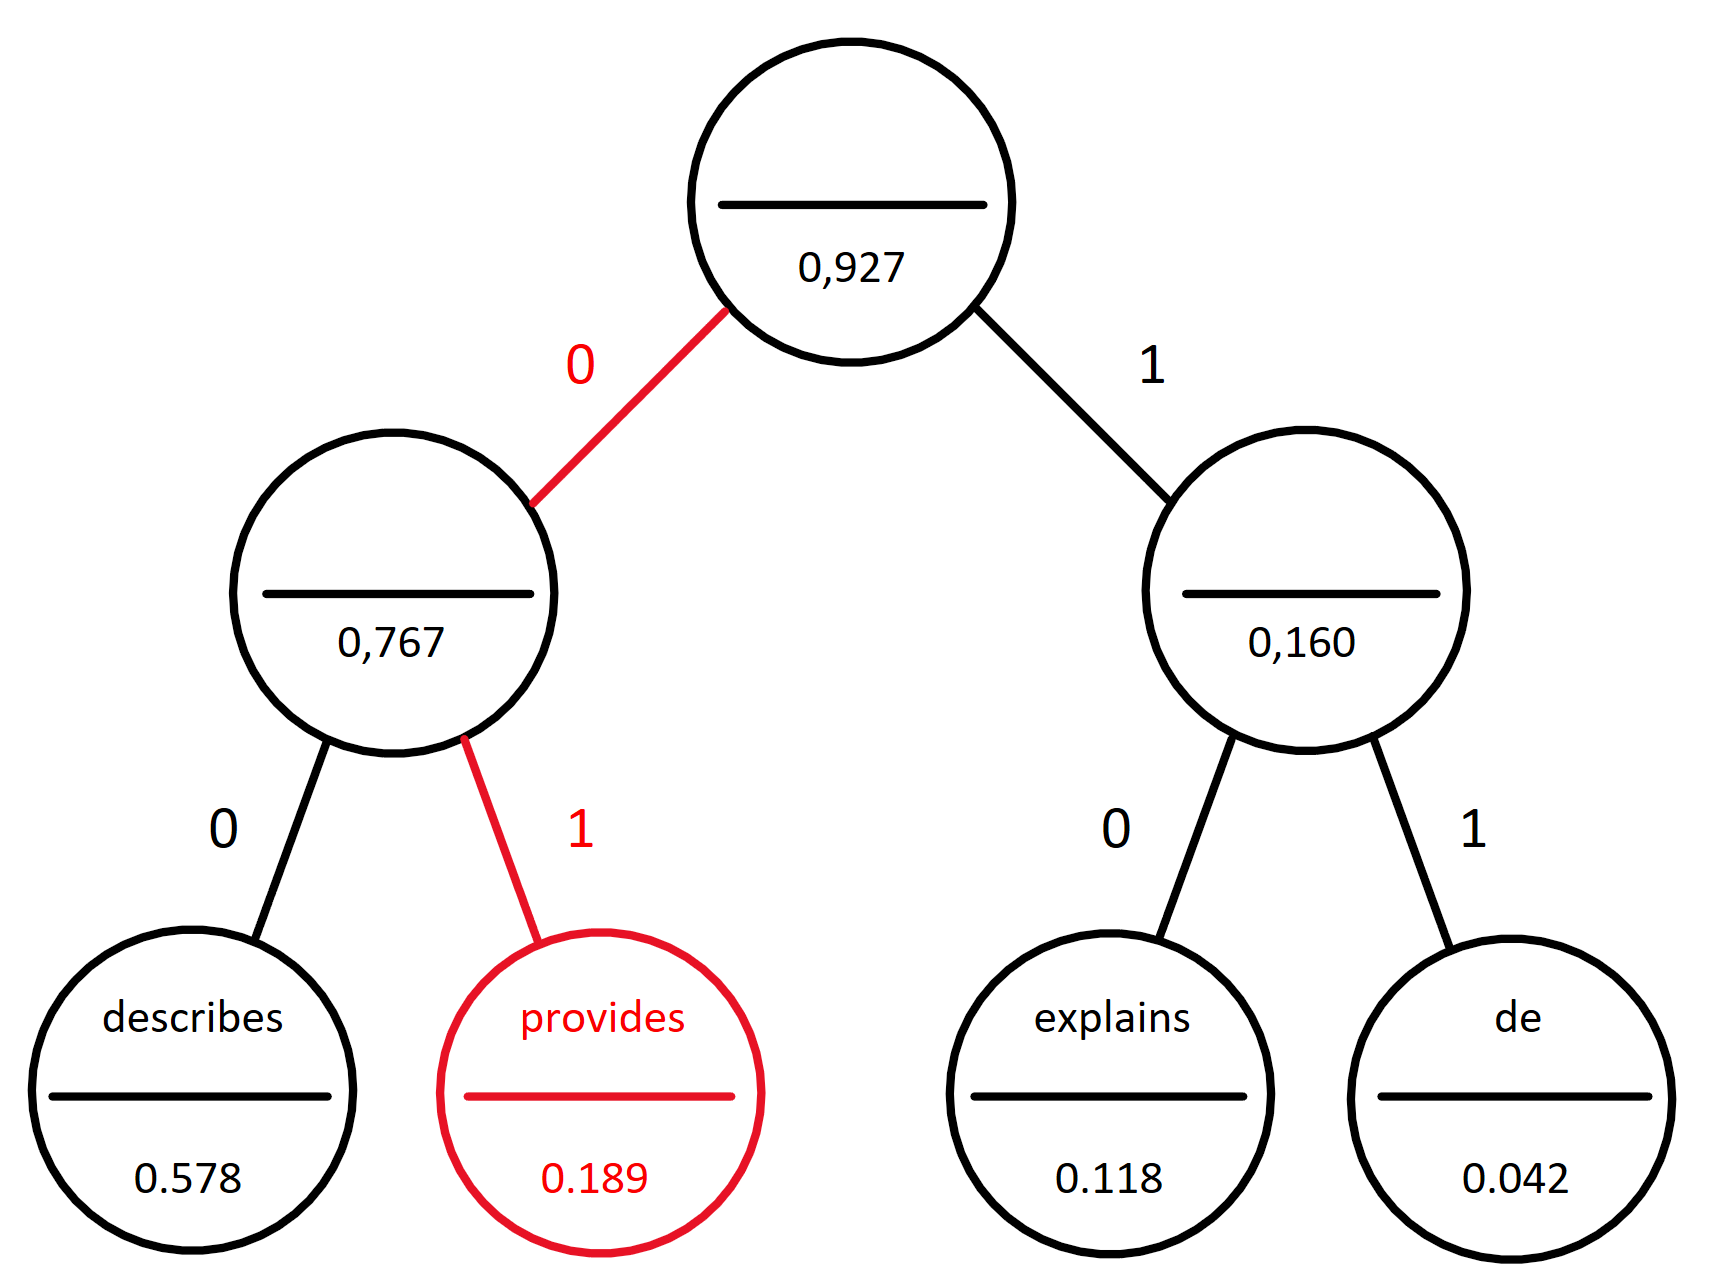
\includegraphics[width=0.67\linewidth]{huffman_coding.png}
		\caption[Huffman coding]{Example of a Huffman tree for \lstinline|bitsPerToken| = 2. Nodes are labelled with tokens and their probabilities, edges with the bits they are interpreted as during traversal. Highlighted is the path that would be taken when encoding the bits 01 of a secret message. The token "provides" would be sampled.}
        \label{fig:huffmanCoding}
    \end{wide}
\end{figure}

This description shows the simplicity of Huffman coding. We only need one parameter to control the trade-off between length and quality of cover texts. A low \lstinline|bitsPerToken| value (e.g. 1 bit/token) will only consider few most likely tokens, making the Huffman tree shallow. Cover texts will be long, but coherent. The inverse is true for a high value (e.g. 4 bits/token). However, Huffman coding also comes with a downside. It aims to maximize cover text quality at maximum compression~\cite{zieglerNeuralLinguisticSteganography2019}. This may be good enough to fool human eavesdroppers, but it is not sufficient to defend against machine-based attacks, as these can identify statistical patterns in cover texts~\cite{zieglerNeuralLinguisticSteganography2019}. This was not the case with Arithmetic coding (see \cref{sec:arithmeticCoding}).

\subsection{Steganography encoding/decoding}
\label{sec:steganographyEncodingDecoding}
The Stegasuras project implemented three steganography algorithms: Arithmetic, Bins and Huffman coding~\cite{zieglerNeuralLinguisticSteganography2019}. We implement Arithmetic and Huffman, dropping Bins entirely. This decision is based on Stegasuras evaluating Bins to perform significantly worse quantitatively and qualitatively, while Arithmetic and Huffman were on par with each other~\cite{zieglerNeuralLinguisticSteganography2019}.

\subsubsection{Arithmetic coding}
\label{sec:arithmeticCoding}
Arithmetic coding commonly refers to a compression algorithm where data is represented as a decimal number in the $ [0, 1) $ interval. This is achieved by iteratively narrowing the boundaries: In every iteration, a sub-interval is selected based on a part of the data and divided into further sub-intervals~\cite{rissanenArithmeticCoding1979}. \cref{fig:arithmeticCoding} provides a visualization. Arithmetic coding is popular because of its ability to compress data to near entropy~\cite{rissanenArithmeticCoding1979}. Stegasuras implements a variant of this using wider integer intervals that don't strictly narrow down to perform steganography~\cite{zieglerNeuralLinguisticSteganography2019,rubinArithmeticStreamCoding1979}.

\begin{figure}
    \begin{wide}
        \captionsetup{width=\linewidth}
        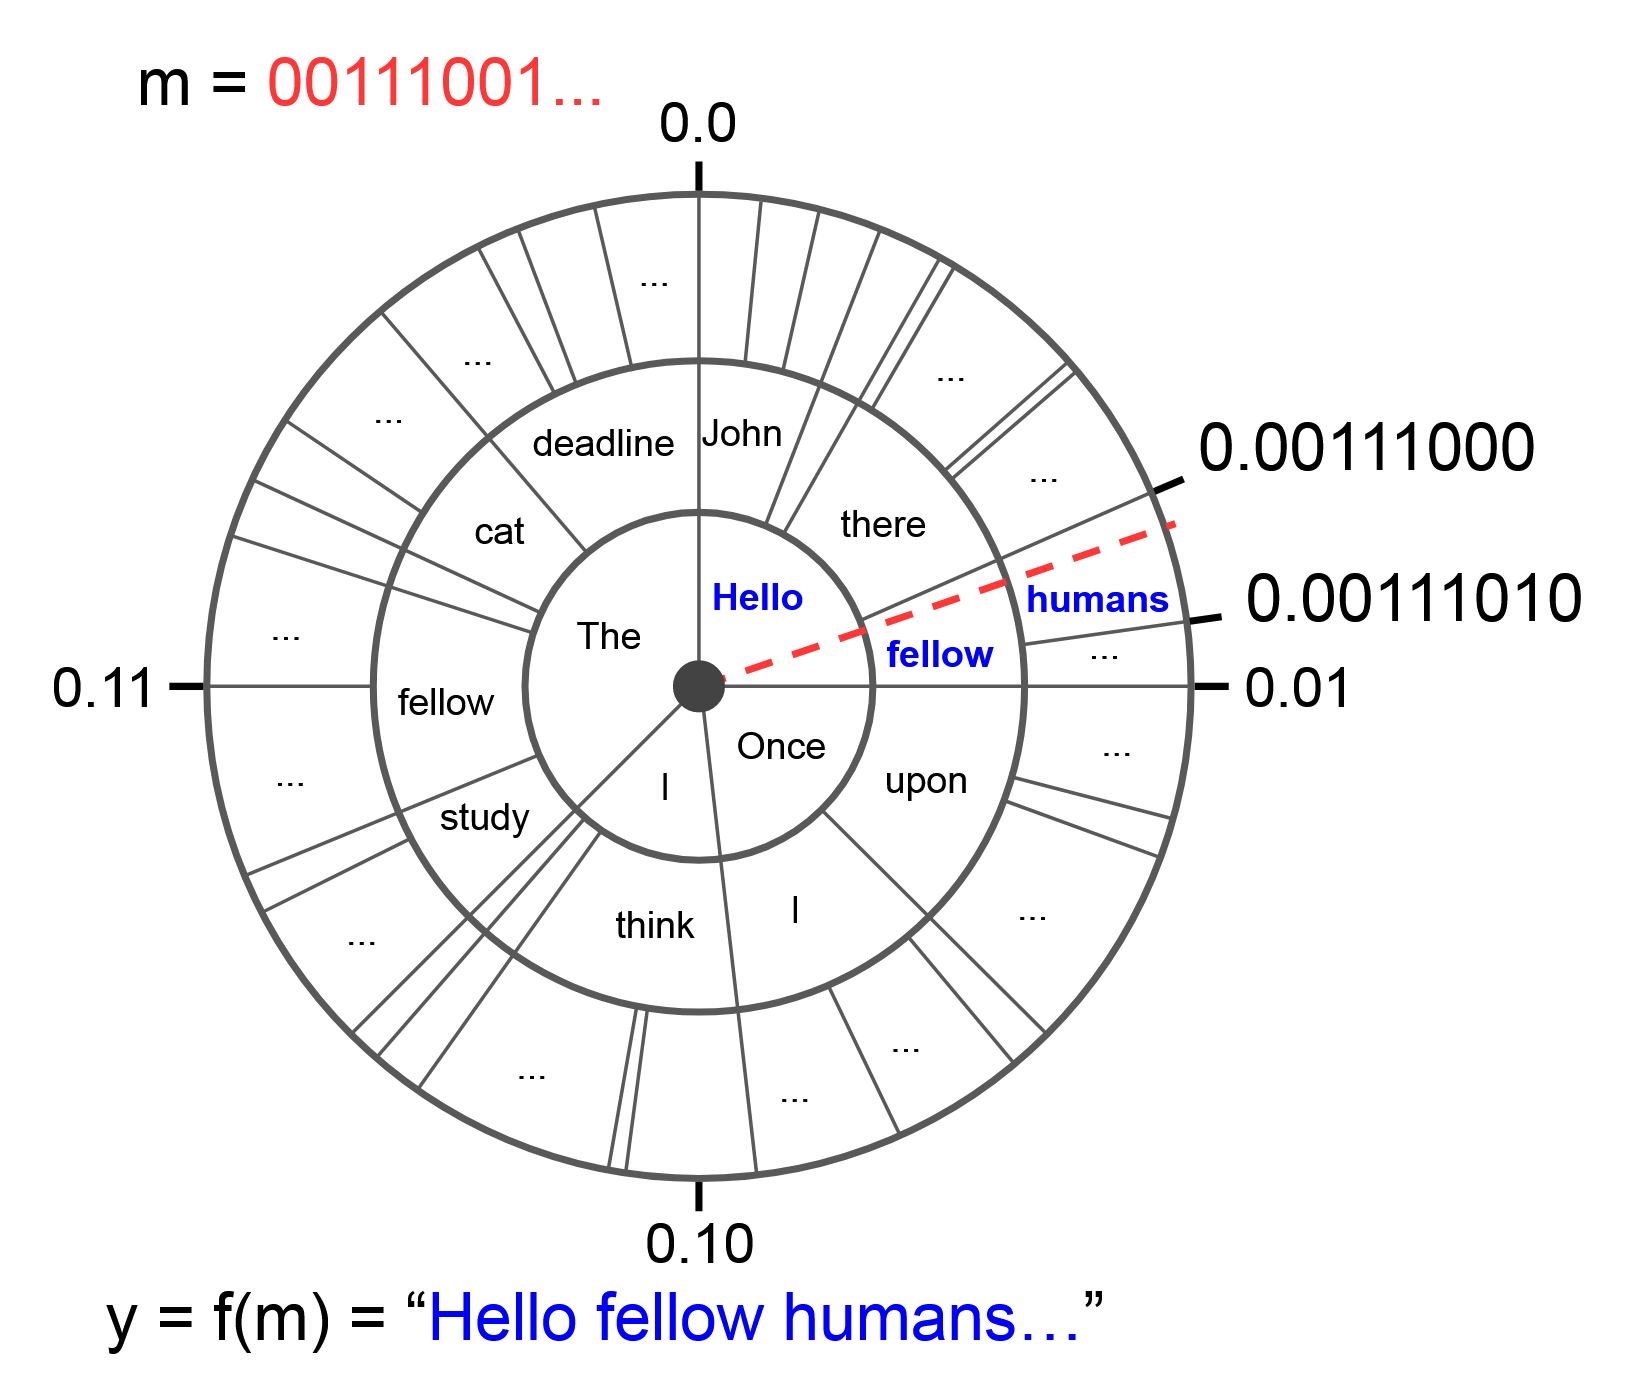
\includegraphics[width=0.75\linewidth]{arithmetic_coding.png}
		\caption[Arithmetic coding]{A visualization of Arithmetic coding. The secret message $m$ gets encoded into a cover text $y$ via a transformation $f$. Iterations are arranged as layers of a circle. The sub-intervals of $ [0, 1) $ get narrower the further they are away from the center. Taken from~\cite{zieglerNeuralLinguisticSteganography2019}.}
        \label{fig:arithmeticCoding}
    \end{wide}
\end{figure}

Arithmetic coding encodes the bits of a secret message into a cover text by sampling specific tokens. This uses the probabilities calculated by the \gls{LLM} and three parameters as input: \lstinline|temperature|, \lstinline|topK| and \lstinline|precision|. The former is a decimal number, the latter two are integers. \lstinline|topK| is a number of tokens not greater than $ n_{vocab} $, the vocabulary size of the \gls{LLM}. \lstinline|precision| is a number of bits. The output is the sampled cover text token.

First, we assign tokens to sub-intervals of an integer interval based on their cumulated probabilities: We define our initial interval as $ [0, 2^{precision}] $. We scale the probabilities by $ 1/temperature $ and sort them in descending order. We only keep the tokens with the top $ min(max(2, n), topK) $ probabilities, where $ n $ is the number of probabilities greater than the inverse width of the current interval. This cuts off any probabilities that would round to 0 in subsequent steps. We rescale the probabilities to the range of the current interval and round them to integers. We cumulate these integer "probabilities" for every token. As those that would round to 0 were cut off, every token now corresponds to a unique integer in the current interval. Interpreting these as upper boundaries effectively assigns every token to a sub-interval.

Then, we sample a cover text token by selecting a sub-interval based on secret message bits: In iteration $ i $, we consider the secret message bits at indices $ i $ to $ i + precision $. If there aren't enough bits left at the end, we do 0-padding. We interpret these bits as an integer and select the sub-interval this integer falls into. Thereby, we sample the token assigned to this sub-interval.

Lastly, we determine how many bits were encoded in iteration $ i $ and calculate the new interval for the next iteration: We convert the boundaries of the selected sub-interval from integer to binary and count the number of most significant bits they share as prefix. This is the number of bits that were encoded in iteration $ i $, so we increment $ i $ by this. This results in the number of most significant bits that are now fixed when representing our secret message as a number in the initial interval. This would narrow our current interval down. As only using the integers within intervals limits resolution, we don't want them to strictly narrow down. Therefore, we manipulate the boundaries. We drop the fixed most significant bits and append as many 1s and 0s as least significant bits to receive the new upper and lower boundaries, respectively. This causes the boundaries to not strictly narrow down, but makes the interval as wide as possible for the next iteration.

This description shows the complexity of Arithmetic coding. In particular, the interplay of \lstinline|topK| and \lstinline|precision| makes their effect on cover text quality hard to estimate. This is not the case with Huffman coding (see \cref{sec:huffmanCoding}). However, Arithmetic coding also comes with a significant strength. It aims to minimize \gls{KL} divergence at maximum compression~\cite{zieglerNeuralLinguisticSteganography2019}. The optimum of no \gls{KL} divergence can be achieved when Arithmetic coding is used with an unmodulated \gls{LLM} (i.e. \lstinline|temperature| = 1.0, \lstinline|topK| = $n_{vocab}$ and \lstinline|precision| = $ \lceil \log_2(topK) \rceil $). This is a powerful defense against machine-based attacks that try to identify statistical patterns in the generated cover texts~\cite{zieglerNeuralLinguisticSteganography2019}. Again, this is not the case with Huffman coding.

\subsubsection{Arithmetic compression}
\label{sec:arithmeticCompression}
Arithmetic compression can be used to convert the secret message from string to binary. It repurposes the Arithmetic coding algorithm we implement for steganography. As this will be explained in \cref{sec:arithmeticCoding}, we only focus on the relevant differences here.

The Stegasuras paper~\cite{zieglerNeuralLinguisticSteganography2019} states that Arithmetic \textit{compression} is Arithmetic \textit{decoding} of the secret message with an empty context. Inversely, it states that Arithmetic \textit{decompression} is Arithmetic \textit{encoding} with an empty context. But this is inconsistent with the Stegasuras code~\cite{zieglerHarvardnlpNeuralSteganography2025}: The context is not \textit{empty}, but consists of an end-of-generation token. With an empty context, the \gls{LLM} would not be able to generate tokens in the first place\footnote{Do not confuse "empty \lstinline|ctx|" (\cref{sec:tokenGenerationWithLlamaCpp}) with "empty context" (here). While the former refers to the \gls{LLM} being given a sensible prompt with no prior chat history, the latter is equivalent to the \gls{LLM} being given an empty string as a prompt. Unfortunately, this ambiguity is unavoidable when sticking to the vocabulary of llama.cpp and Stegasuras, respectively.}. Furthermore, Arithmetic compression doesn't call the encode/decode functions with the same arguments as Arithmetic coding does: \lstinline|temperature| is fixed to 1.0, \lstinline|topK| is fixed to the vocabulary size of the \gls{LLM}, and \lstinline|precision| is set as high as possible (62 bits in our implementation to avoid overflows). This forces the unmodulated \gls{LLM} to use as much of its vocabulary as possible in every iteration of the algorithm.

We make a small modification to the algorithm as implemented in Stegasuras, which is only relevant for compression. To clean up artefacts that may be generated during decoding of a cover text, we need to be able to sample the ASCII NUL character as a token (see \cref{sec:finishingTheLastSentence}). Arithmetic coding involves assigning tokens to sub-intervals of $ [0, 2^{precision}) $ before sampling them (see \cref{sec:arithmeticCoding}). To ensure ASCII NUL can always be sampled, we assign it to the last sub-interval. This is similar to more general implementations of Arithmetic compression, where the last sub-interval is interpreted as end-of-file to terminate the algorithm.

Arithmetic compression is probabilistic. It relies on the \gls{LLM} to predict the secret message token-wise (see \cref{sec:arithmeticCoding}). As the secret message is arbitrary user input, the \gls{LLM} may not be able to predict it. This makes Arithmetic compression slightly prone to failures. However, Arithmetic compression doesn't need to store any metadata about the secret message to be able to decompress it again. This is a benefit over many other compression algorithms, as it significantly reduces attack surface. Huffman compression is a counterexample.

\section{Finishing the last sentence}
\label{sec:finishingTheLastSentence}
Our app is based on the Stegasuras project~\cite{zieglerNeuralLinguisticSteganography2019}. While we are able to use its algorithms for steganography, they come with an unsolved edge case. If cover text generation would stop as soon as the secret message is encoded, the last sentence would most likely be incomplete. Not finishing the last sentence is not an option, as it would make our communication highly suspicious to an attacker. A possible solution is performing greedy sampling until a suitable punctuation mark is reached. This is already demonstrated in Stegasuras~\cite{zieglerHarvardnlpNeuralSteganography2025}. But if we decode such a cover text, we get the secret message, followed by some noise. This is because the tokens from greedy sampling don't encode any actual information. Our app would provide a rather unpolished user experience if we left it like this.

We propose a solution to clean up this noise during decoding: A suitable stop signal is injected somewhere in the encoding process, appending it to the secret message. During decoding, we can thereby identify the end of the secret message. Any noise following the stop signal can then be cut off. The challenge is finding a step in the encoding process suitable for injection, which also determines the form of the stop signal.

We briefly recall how the secret message is encoded: First it gets converted from string to binary, compressing it in the process. Then it gets encoded into a cover text using the algorithm-specific sampling, followed by greedy sampling. It may also get encrypted between compression and cover text generation. Therefore, we cannot make any structural assumptions about the bit sequence being \textit{decoded} from the cover text. We have to insert our stop signal earlier in the encoding process, so that we can identify it later in the decoding process.

This ultimately led us to consider a special character as a stop signal. We append this special character to the secret message before it gets converted from string to binary. A suitable special character needs to be unlikely as organic user input, so that blocking it doesn't degrade the user experience significantly. The ASCII NUL character presents such a solution. While languages such as C and C++ use it for string termination, it doesn't serve any purpose in Kotlin. It doesn't have a visual representation either, and therefore is not on any standard keyboard. When appending it to the secret message, it introduces a small maximum overhead of 8 bits if UTF-8 is used for binary conversion. When the secret message is being compressed, the overhead is even less.

\section{Creating a conversation between cover texts}
\label{sec:creatingAConversationBetweenCoverTexts}
A \gls{LLM} fundamentally works by completing any prompt it is given (see \cref{sec:tokenGenerationWithLlamaCpp}). We are already able to leverage this for steganography by manipulating token generation, thereby encoding a secret message into a cover text (see \cref{sec:steganographyEncodingDecoding}). But we still don't have a way to create a conversation between cover texts. This means our first requirement (see \cref{ch:introduction}) is not fulfilled yet.

This section will show how creating a conversation between cover texts is possible. We will also show how to influence the \gls{LLM} behaviour on a lower level, via a system prompt. Both is achieved at once, by formatting the context as a conversation using special tokens~\cite{jiangChatBugCommonVulnerability2025}.

The context is formatted into a conversation by structuring it into messages. Each message has a role and a content~\cite{jiangChatBugCommonVulnerability2025}. There are three possible roles: System, user and assistant~\cite{jiangChatBugCommonVulnerability2025}. The system role is reserved for the system prompt. Its content is a natural language command the user can give the \gls{LLM} to influence its behaviour~\cite{jiangChatBugCommonVulnerability2025}. For the \gls{LLM}, the system prompt is always the first message of the conversation. In a typical \gls{UI} however, the system prompt is hidden away in the settings. Our implementation handles it like this too.

The user role is assigned to the subsequent prompts input by the user~\cite{jiangChatBugCommonVulnerability2025}. The assistant role is assigned to the responses output by the \gls{LLM}~\cite{jiangChatBugCommonVulnerability2025}. At the end of the formatted context, the special token for the assistant role is appended. This signals the \gls{LLM} to continue the conversation, i.e. to respond to the last message. Listing~\ref{lst:chatTemplate} shows an example.

% Add some space on top of listing to match bottom
\vspace{0.25cm}

\begin{lstlisting}[caption={[llama.cpp: Chat templates]{Example for a context formatted with the chat template of Llama 3.2 1B. Some line breaks have been added for readability.}}, label={lst:chatTemplate}]
<|start_header_id|>system<|end_header_id|>Let's do a role play. You and I are friends, texting with each other. We talk about what we did on the weekend. Be brief and casual, but friendly and engaging. Use emojis and phrases typical for chat messages.<|eot_id|>
<|start_header_id|>user<|end_header_id|>How was your weekend?<|eot_id|>
<|start_header_id|>assistant<|end_header_id|>
\end{lstlisting}

Unfortunately, the special tokens for context formatting are not uniform across \glspl{LLM}. Fortunately, llama.cpp has support for a wide range of formattings. In the vocabulary of llama.cpp, they are called chat templates~\cite{gerganovGgerganovLlamacpp2024,jiangChatBugCommonVulnerability2025}. We can query a \gls{LLM} for its chat template and pass this as a parameter to other functions. Thereby, we remain compliant with our fourth requirement of making the \gls{LLM} swappable (see \cref{ch:introduction}).

When completing the formatted context, the \gls{LLM} performs our algorithm-specific sampling (see \cref{sec:algorithms}). In doing so, we encode information in the next chat message and create a conversation from cover texts. Finally, our first requirement is fulfilled.

Strictly speaking, the conversation doesn't need to consist only of \textit{cover texts}. It may as well be composed of an arbitrary mixture of cover texts and plain texts, i.e. messages that don't encode a secret message. Our app allows this by letting the user toggle steganography on/off on the conversation screen (see \cref{sec:conversationScreen}). This gives the user great freedom to steer the topic of the conversation by sending plain text messages for non-sensitive communication. In addition to the system prompt, this enables us to improve cover text quality further.

Lastly, we mentioned that the \gls{LLM} needs to be able to talk \textit{to itself} (see \cref{sec:howToSelectASuitableLLM}). What we mean by this is that the \gls{LLM} is used by both chat partners to generate cover texts that are replies to the other chat partner. Consider this example: We have two chat partners, Alice and Bob. Alice wants to send a new cover text to Bob. The prior messages in the conversation are used as context. For encoding, Alice's prior messages have to be assigned the assistant role and Bob's prior messages have to be assigned the user role. When Bob receives this cover text, he has to replicate this state to decode it. When Bob wants to reply with another cover text, the roles are inversed. For encoding, Bob's prior messages have to be assigned the assistant role and Alice's prior messages have to be assigned the user role. Alice has to replicate this state to decode it. The roles are constantly switched following this pattern, effectively making the \gls{LLM} talk to itself without knowing it.

\section{Emojis}
\label{sec:emojis}
Emojis are widely used in instant messaging to express emotions, add visualizations or draw attention~\cite{zhouGoodbyeTextHello2017}. Being able to enrich our cover texts with this form of non-verbal communication is essential to make them seem organic. Today's \glspl{LLM} are able to output emojis when being prompted to (see \cref{sec:howToSelectASuitableLLM}). By demanding emojis in the system prompt, our app is able to do this as well. Accomplishing this however required some attention to detail. Therefore, we explain what needs to be considered when working with emojis and other non-ASCII characters in the context of the \gls{JNI} (see \cref{sec:javaNativeInterface}).

The \gls{JNI} is used to pass parameters between our Kotlin and C++ code. This requires conversions between the corresponding data types. For most data types this is simple, but for strings this is more sophisticated. This is due to collisions between different character encodings. As the ASCII encoding is contained in virtually all other encodings, pure ASCII strings generally are interoperable~\cite{gleaveMakingCompressionAlgorithms2017}. While the ASCII character set is sufficient for basic communication in English, it doesn't include emojis.

Emojis require the full Unicode character set. This can be encoded in various ways, the most common being UTF-8~\cite{gleaveMakingCompressionAlgorithms2017}. Consider the implementation of the \lstinline|LlamaCpp.detokenize| function in our source code: It detokenizes an array of token IDs back into a string using the \gls{JNI}. On the C++ side, one might be tempted call the \lstinline|NewStringUTF| function to create a \lstinline|jstring| object to pass back to Kotlin. While this works fine for ASCII strings, it makes our app crash when working with emojis. This is due to a \textit{modified} UTF-8 encoding being used by Java and therefore by the \gls{JNI}~\cite{oracleJNIFunctions}. To bypass this, we return the UTF-8 encoding of a string as a \lstinline|jbyteArray| instead. On the Kotlin side, we explicitly call the String constructor to specify that the bytes are UTF-8. This abstracts any Kotlin internals away.

While emojis now enable us to improve cover text quality, they introduce some further difficulties. When finishing the last sentence of the cover text during encoding, we use greedy sampling and terminate when reaching a suitable punctuation mark (see \cref{sec:finishingTheLastSentence}). To fulfill the third requirement defined in \cref{ch:introduction}, we have to keep cover texts as short as possible. If a cover text contains emojis, they may be used in place of punctuation marks to end a sentence~\cite{zhouGoodbyeTextHello2017}. But unlike punctuation marks, emojis cannot easily be detected using the Kotlin standard library. A simple approach like detecting non-ASCII characters would already conflict with the German letters ä, ö and ü, for example. A more sophisticated approach was implemented, using regular expressions to detect the Unicode categories containing emojis. But this didn't yield satisfying results as it corrupted a significant portion of cover texts. Therefore, cover texts including emojis only end when an appropriate punctuation mark is generated. This possibly makes them longer than necessary. But we consider it worth the trade-off, as the use of emojis can be easily influenced via the system prompt.
